\documentclass[a4paper]{article} 
\usepackage[longend,ruled,linesnumbered]{algorithm2e}
\addtolength{\hoffset}{-2.25cm}
\addtolength{\textwidth}{4.5cm}
\addtolength{\voffset}{-3.25cm}
\addtolength{\textheight}{5cm}
\setlength{\parskip}{0pt}
\setlength{\parindent}{0in}

%----------------------------------------------------------------------------------------
%	PACKAGES AND OTHER DOCUMENT CONFIGURATIONS
%----------------------------------------------------------------------------------------

\usepackage{blindtext} % Package to generate dummy text
\usepackage{charter} % Use the Charter font
\usepackage[utf8]{inputenc} % Use UTF-8 encoding
\usepackage{microtype} % Slightly tweak font spacing for aesthetics
\usepackage[italian]{babel} % Language hyphenation and typographical rules
\usepackage{amsthm, amsmath, amssymb} % Mathematical typesetting
\usepackage{float} % Improved interface for floating objects
\usepackage[final, colorlinks = true, 
            linkcolor = black, 
            citecolor = black]{hyperref} % For hyperlinks in the PDF
\usepackage{graphicx, multicol} % Enhanced support for graphics
\usepackage{xcolor} % Driver-independent color extensions
\usepackage{marvosym, wasysym} % More symbols
\usepackage{rotating} % Rotation tools
\usepackage{censor} % Facilities for controlling restricted text
\usepackage{listings, style/lstlisting} % Environment for non-formatted code, !uses style file!
\usepackage{pseudocode} % Environment for specifying algorithms in a natural way
\usepackage{style/avm} % Environment for f-structures, !uses style file!
\usepackage{booktabs} % Enhances quality of tables
\usepackage{tikz-qtree} % Easy tree drawing tool
\tikzset{every tree node/.style={align=center,anchor=north},
         level distance=2cm} % Configuration for q-trees
\usepackage{style/btree} % Configuration for b-trees and b+-trees, !uses style file!
\usepackage[backend=biber,style=numeric,
            sorting=nyt]{biblatex} % Complete reimplementation of bibliographic facilities
\addbibresource{ecl.bib}
\usepackage{csquotes} % Context sensitive quotation facilities
\usepackage[yyyymmdd]{datetime} % Uses YEAR-MONTH-DAY format for dates
\renewcommand{\dateseparator}{-} % Sets dateseparator to '-'
\usepackage{fancyhdr} % Headers and footers
\pagestyle{fancy} % All pages have headers and footers
\fancyhead{}\renewcommand{\headrulewidth}{0pt} % Blank out the default header
\fancyfoot[L]{} % Custom footer text
\fancyfoot[C]{} % Custom footer text
\fancyfoot[R]{\thepage} % Custom footer text
\newcommand{\note}[1]{\marginpar{\scriptsize \textcolor{red}{#1}}} % Enables comments in red on margin



\usepackage{amsmath}
\usepackage{amsfonts}
\usepackage{tcolorbox}
%----------------------------------------------------------------------------------------

\usepackage{graphicx}
% \usepackage[table,xcdraw]{xcolor}
\usepackage{multirow}
\tcbuselibrary{theorems}

\newtcbtheorem[]{teorema}{}%
{colback=gray!15,colframe=gray!70}{th}

\begin{document}

%-------------------------------
%	TITLE SECTION
%-------------------------------

\fancyhead[C]{}
\hrule \medskip % Upper rule
\begin{minipage}{0.295\textwidth} 
\raggedright
\footnotesize
Andrei Gabriel Taraboi \hfill\\   
\hfill\\
\end{minipage}
\begin{minipage}{0.4\textwidth} 
\centering 
\large 
Machine Learning\\ 
\normalsize 
\end{minipage}
\begin{minipage}{0.295\textwidth} 
\raggedleft
\hfill\\
\end{minipage}
\medskip\hrule 
\bigskip

%-------------------------------
%	CONTENTS
%-------------------------------
\tableofcontents

\newpage
\part{Teoria}
%%%%%%%%%%%%%%%%%%%%Lezioni
\section{Lezione 1 e 2}
Un \textbf{sistema di apprendimento automatico} ricava da un \textit{dataset} una conoscenza non fornita a priori, descrivendo dati non forniti in precedenza. Si estrapolano informazioni facendo assunzioni sulle informazioni sistema già conosciute, creando una \textbf{classe delle ipotesi H}. Si cercano ipotesi coerenti per guidare il sistema di apprendimento automatico. Bisogna però mettere in conto anche eventuali errori, cercando di capire se esiste davvero un'ipotesi coerente e, in caso di assenza, si cerca di approssimare. In quest'ottica bisogna mediare tra \textbf{fit} e \textbf{complessità}. Ogni sistema dovrà cercare di mediare tra questi due aspetti, un \textit{fit} migliore comporta alta \textit{complessità}. Si ha sempre il rischio di \textbf{overfitting}, cercando una precisione dei dati che magari non esiste.\\
    
Abbiamo inoltre una \textbf{ipotesi da apprendere \textnormal{o} concetto target(o label}: tra tutte le ipotesi possibili, viene identificata, grazie ai dati di addestramento, quella giusta. Possiamo facilmente capire invece cosa intendiamo per \textbf{target dell’addestramento}, corrisponde alla risposta che ci si aspetta sull’istanza. Se l’ipotesi non mi fornisce come risposta il target di addestramento, allora la posso scartare. Altrimenti si definisce ipotesi accettabile o valida.

Definiamo alcuni concetti base: 
\begin{itemize} 
    \item \textbf{task (\textit{T})}, il compito da apprendere. È più facile apprendere attraverso esempi che codificare conoscenza o definire alcuni compiti. Inoltre il comportamento della macchina in un ambiente può essere diverso da quello desiderato, a causa della mutabilità dell'ambiente ed è più semplice cambiare gli esempi che ridisegnare un sistema.
    \item \textbf{performance (\textit{P})}, la misura della bontà dell'apprendimento.
    \item \textbf{experience (\textit{E})}, l'esperienza sui cui basare l'apprendimento. Il tipo di esperienza scelto può variare molto il risultato e il successo dell'apprendimento. 
\end{itemize}

In merito alle parti software distinguiamo: il
  \textbf{learner}, ovvero la parte di programma che impara dagli esempi in modo   automatico e il  \textbf{trainer}, il \textit{dataset} che fornisce esperienza al \textit{learner}

L'ipotesi da apprendere viene chiamata \textbf{concetto target} (tra tutte le ipotesi possibili identifico quella giusta dai dati di addestramento).

Si hanno inoltre diversi tipi di apprendimento: 
    \begin{itemize}
        \item \textbf{apprendimento supervisionato}, dove vengono forniti a priori esempi di comportamento e si suppone che il \textit{trainer} dia la risposta corretta per ogni input. L'esperienza è fornita da un insieme di coppie: \[S\equiv\{(x_1,y_1),(x_2,y_2),\ldots,(x_n,y_n)\}\] e, per ogni input ipotetico $x_i$ l'ipotetico trainer restituisce il corretto $y_i$ (target). Ci ritroviamo in questo caso se all'interno delle istanze, se c'è target.
        \item Se riceviamo istanze di addestramento senza label/target ci ritroviamo nel tipo di \textbf{apprendimento non supervisionato}. In un 
            \textbf{L'apprendimento non supervisionato} l’esperienza di apprendimento è rappresentata da esempi “non classificati”: non esiste un trainer che fornisce le risposte corrette agli input. Non c'è target e si ha \textit{libertà di classificazione}. Si cerca una \textit{regolarità} e una \textit{struttura} insita nei dati. In questo caso si ha:  \[S\equiv\{x_1,x_2,\ldots,x_n\}\]
        \item \textbf{Apprendimento per rinforzo} Il learner interagisce con l’ambiente e riceve una ricompensa positiva o negativa . Si lavora con un \textit{addestramento continuo}, aggiornando le ipotesi con l'arrivo dei dati. Durante la fase di test bisogna conoscere le prestazioni e valutare la correttezza di quanto appreso. Il learner viene addestrato tramite \textit{rewards} e quindi apprende una strategia per massimizzare i \textit{rewards}, detta \textbf{strategia di comportamento} e per valutare la prestazione si cerca di massimizzare a lungo termine la ricompensa complessivamente ottenuta.
    \end{itemize}
    
Si avrà, in realtà, a che fare con dati, di target e ipotesi, booleani e questo ambito è propriamente chiamato \textbf{concept learning}. In questo contesto si cerca di capire quale funzione booleana è adatta al mio addestramento. Traduciamo il dominio reale in valori booleani. 

Introduciamo quindi il \textbf{bias induttivo} considerando:
\begin{itemize}
  \item un algoritmo di learning del concetto $L$
  \item degli esempi di training $D_C=\{\langle x,c(x)\rangle\}$
\end{itemize}
Dove la funzione target associa ad ogni istanza un valore in $\{0,1\}$, appunto booleano. Una classe di ipotesi H è data da vincoli sugli attributi. Il training set D è costituito da esempi positivi e negativi della funzione target, dove $x$ è la nostra istanza, e $c(x)$ corrisponde al valore associato dalla funzione target a quell’istanza. Un’ipotesi appartiene alla classe di ipotesi se ogni istanza del training set è tale che il valore della funzione target sull’istanza coincide con il valore predetto dall’ipotesi.


\subsection{Algoritmi di apprendimento}
\subsubsection{Rote leaner}
La macchina è programmata per mantenere una cronologia dei calcoli e confrontare il nuovo input con la sua cronologia degli input e degli output, recuperando l'output memorizzato se presente. Questo modello richiede che la macchina possa essere modellata come una funzione, producendo sempre lo stesso output per lo stesso input, e può essere formalmente descritto come segue: \\
$ f({\displaystyle \ x_{1},x_{2}, \dots ,x_{n}})\to \ ({\displaystyle \ y_{1},y_{2},\dots ,y_{p}})\ \to store (({\displaystyle \ x_{1},x_{2},...,x_{n}}),({\displaystyle \ y_{1},y_{2},...,y_{p}})$
Non si un inductive bias. 
\subsubsection{Version space candidate elimination}
Sia G l'insieme di ipotesi massimamente generali in H, e S l'insieme di ipotesi massimamente specifiche in H. Per ciascun esempio di trainging \textit{\textbf{d}}:
\begin{itemize}
    \item Se \textbf{\textit{d}} è positivo
        \begin{itemize}
            \item togli da G ipotesi inconsistenti con \textit{\textbf{d}}
            \item UPDATE-S: per ciascuna ipotesi s in S che non è consistente con d, togli s da S e aggiungi a S tutte le minime generalizzazioni h di s tali che: h è consistente con d e alcuni membri di G sono più generici di h. Successivamente rimuovi da S ogni ipotesi che è più generale di un'altra ipotesi in S.
        \end{itemize}
    \item Se \textbf{\textit{d}} è negativo eseguo,\begin{itemize}
        \item togli da S ipotesi inconsistenti con \textit{\textbf{d}}
            \item UPDATE-G: per ciascuna ipotesi g in G che non è consistente con d, togli g da G e aggiungi a S tutte le minime specializzazioni h di g tali che: h è consistente con d e alcuni membri di S sono più generici di h. Successivamente rimuovi da G ogni ipotesi che è meno generale di un'altra ipotesi in G.
        \end{itemize}
\end{itemize}
Questo include solamente il discorso di \textbf{Candidate Elimination}, per quanto riguarda invece \textbf{Version Space}, possiamo affermare che è costituito da serie di ipotesi tra quelle possibili nella classe d’ipotesi che hanno specificato un set di istanze (training set) e che sono consistenti su quegli esempi.\\ L’assunzione fondamentale, quando si fa riferimento al Candidate Elimination, è che qualunque ipotesi scelta per azzeccare gli esempi di addestramento, sia abbastanza buona anche nella fase di test, ovvero con gli esempi che non si sono ancora visti.
\subsubsection{Find-S}
Lo spazio delle ipotesi è descritto da congiunture (operazioni di AND) tra attribuiti. 
Questo algoritmo permette di partire dall'ipotesi più specifica  e generalizzarla, trovando ad ogni passo un'ipotesi più specifica e consistente con il training set $D$. \\
L'ipotesi in uscita sarà anche consistente con gli esempi negativi dando prova che il target è effettivamente in $H$. Con questo algoritmo non si può dimostrare di aver trovato l'unica ipotesi consistente con gli esempi e ignorando gli esempi negativi non posso capire se $D$ contiene dati inconsistenti. In altre parole il risultato dice che, se l’ipotesi segreta è una congiunzione e si è scelta quella più aderente alle istanze positive, allora le istanze al di fuori sono per forza negative.
\section{Lezione 3}
\subsection{Decioson Tree}
Tornando a parlare di concept learning, possiamo utilizzare un altro metodo di rappresentazione dei dati , al posto delle classiche funzioni booleane, \textbf{alberi di decisione} per rappresentare un modello che applicato ad esempi non visti ci dirà se applicare in output un'etichetta vera o falsa in base a quanto appreso. Siamo in ambito di \textbf{apprendimento supervisionato}.\\ 
Un albero di decisione è costruito in modo che ad ogni nodo interno controlla un attributo, ogni ramo corrisponde al valore di un attributo e ogni foglia assegna una classificazione (Si/No). Aggiungiamo anche che si esistono attributi che hanno anche più di due valori\textbf{}

Possiamo dire che gli alberi decisionali descrivono tutte le funzioni booleane. Avendo $n$ funzioni booleane avremo un numero distinto di tabelle di verità (e quindi di alberi decisionali), ciascuna con $2^n$ righe, pari a $2^{2^{n}}$.\\
Riassumiamo alcune caratteristiche degli alberi decisionali:
\begin{itemize}
  \item abbiamo attributi con valori discreti, che possiamo elencare
  \item abbiamo un target di uscita discreto, le foglie hanno valori precisi
  \item posso costruire ipotesi anche con disgiunzioni 
  \item può esserci rumore nel training dei dati, cioè i dati non hanno sempre una corretta corrispondenza istanza e valore target da attribuire
  \item possono esserci attributi di cui non ho informazioni
\end{itemize}
\subsection{Algoritmo ID3}
L'idea di base è trovare un albero piccolo di partenza, scelto tra i tanti alberi disponibili, e applicare un criterio di crescita dell'albero che sia sempre coerente con le istanze ricevute in addestramento. Si punta ad arrivare ad un albero valido per tutti gli esempi ricevuti e anche per quelli non visti

L'algoritmo prevede la scelta di un un attributo A, che denomineremo come il ``miglior'' attributo di decisione per il prossimo nodo. Quindi ci serve un buon attributo secondo il quale dividere le istanze è uno che divide le negative dalle positive.
Per eseguire la decisione introduciamo il seguente concetto : [$esempi \ positivo+, esempi \ negativo-$], entrambi rappresentati con un valore intero. Gli esempi positivi sono gli esempi che già mi hanno restituito \textit{yes} mentre quelli negativi mi hanno restituito \textit{no}. In generale sono tutti esempi su cui devo ancora valutare l'attributo. E proseguo così assegnando etichette positive e negative.
\newline

Per ora stabiliamo ad occhio lo sbilanciamento, in base alle etichette positive e negative.\\ Il criterio di scelta ci porta a preferire lo sbilanciamento, preferendo, in modo ideale, un subset con \textit{tutti positivi} o \textit{tutti negativi}. Quindi se un attributo ha divisioni sbilanciate è da ritenersi migliore.

\subsection{Entropia}
Sia S un training set, con possibili valori $v_i$ con $i = 1 \dots n$, se l’entropia di un insieme di bit misura più o meno la sua quantità di informazione, si può richiamare la seguente formula: $$I(P(v_1),\dots,P(v_n))=\displaystyle \sum_{i=1}{-P(v_i)\log_2P(v_i)}$$
Dove:
\begin{itemize}
    \item $I(valore)$ indica il valore dell'entropia sul valore preso in considerazione
    \item $v_i$  sono i possibili valori assumibili dalle istanze del training set
    \item $P(v_i)$ è la probabilità che un’istanza assuma quel valore.
\end{itemize}

Nella variabile $p$ conto i valori di $S$ con etichetta positiva e con $n$ negativa (esempi positivi e negativi). Se inoltre diciamo che $p_+$ è la proporzione di esempi positivi e $p_-$ di quelli negativi (saranno quindi tra 0 e 1) possiamo misurare l'\textbf{impurità} (la confusione) contenuta in $S$ con l'entropia: $Entropy(S)=-p_+\log_2 p_+-p_-\log_2 p_-$
\\
Se l’entropia è alta, è perché le istanze sono ben divise tra positive e negative, se è bassa è perché sono tutte o positive o negative e quindi ho poche informazioni.
Parliamo quindi di \textbf{information gain} $IG$ che viene calcolato su ogni attributo $A$ e su $S$: \[IG(S,A)=I\left(\frac{p}{p+n},\frac{n}{p+n}\right)-remainder(A)\] dove: 
\[remainder(A)=\sum_{i=1}^v \frac{p_i+n_i}{p+n}I\left(\frac{p_i}{p_i+n_i},\frac{n_i}{p_i+n_i}\right)\] 
e quindi l'information gain è la riduzione aspettata nell'entropia per ordinare $S$ sull'attributo $A$. Per scegliere l’attributo migliore per ogni nodo si utilizza l’information gain (IG più alto).


Facciamo qualche osservazione finale sull'\textbf{algoritmo ID3}:
\begin{itemize}
  \item lo spazio delle ipotesi è completo e sicuramente contiene il target
  \item ho in output una singola ipotesi
  \item non si ha backtracking sugli attributi selezionati, si procede con una ricerca greedy (ma trovo scelte buone localmente e non ottime)
  \item fa scelte basate su una ricerca statistica, facendo sparire incertezze sui dati
  \item il bias non è sulla classe iniziale, essendo lo spazio delle ipotesi completo, ma sulla scelta di solo alcune funzioni, preferendo alberi corti (e più semplici) e posizionando attributi ad alto information gain vicino alla radice. 
  \item $H$ è l'insieme potenza delle istanze $X$
\end{itemize}

\subsection{Overfitting}

Viene introdotto però l'\textbf{overfitting}. Se misuro l'errore di una ipotesi $h$ sul training set ($error_{traini}(h)$) e poi misuro l'errore di quella ipotesi sull'intero set delle possibili istanze $D$ ($error_D(h)$) ho che l'ipotesi $h$ va in \textbf{overfit} sul quel data set se: 
$$error_{train}(h) < error_{train}(h') \land error_D(h)>error_D(h')$$
Cosa possiamo fare per evitare l’overfitting? \textbf{pruning}, potatura dopo aver addestrato un albero completo oppure 
\textbf{Misura di complessità delle ipotesi}: MDL (Minimum Description Length)
\section{Reti Neurali}
Data la potenza potenza del calcolo elettronico, infatti si è capaci di eseguire calcoli numerici complessi (anni per un uomo) in frazioni di secondo l memorizzazione grandi quantità di data, bisogna. Questa potenza di calcolo ha però diversi limiti, come il riconoscimento accurati di persone oggetti e suoni in presenza di rumore.  \\
Per cercare di superare questo problema, si potrebbe addestrare questa potenza di calcolo attraverso le reti neurali. 

\subsection{Neuroni formali}
Per i neuroni formali utilizziamo un modello matematico. Questo modello matematico è stato proposto da \textbf{McCulloch} e \textbf{Pitts} e definisce formalmente un \textbf{neurone binario a soglia} come una quadrupla: \[\langle n, C, W, \theta \rangle\] dove: 
\begin{itemize} 
    \item $n$ specifica il \textbf{nome} del neurone stesso, una sorta di identificativo \item $C$ specifica l'\textbf{insieme degli input} $c_i$ 
    \item $W$ specifica il \textbf{vettore dei pesi} $w_i$, associati ad ogni input $c_i$. È una rappresentazione formale dei pesi delle sinapsi (e si nota che possono essere sia positivi che negativi) 
    \item $\theta$ specifica la \textbf{soglia}, utile per definire quando un neurone manda effettivamente il segnale
\end{itemize}

Per definire i due stati del neuroni si usa l'insieme dei valori $\{0,1\}$ oppure l'insieme \{-1,1\}, si ha infatti un neurone binario. Inoltre avendo il vettore $w_i$ di pesi, per gli input
siamo in grado di definire la funzione di transizione, dove viene riportato il concetto di soglia (effetto soglia): 
$s(t+1)=1 \mbox{ \textnormal{sse} }\sum w_i\cdot s_i(t)\geq \theta$

La formula indica che in un tempo successivo $t+1$ (con $s(t)$ che definisce uno $stato$ al tempo $t$) ho che il neurone emette il segnale (stato pari ad 1) sse al tempo precedente $t$ ho avuto una somma pesata degli input $c_i(t)$ maggiore della soglia $\theta$. (l'output del neurone rappresenta quindi il suo stato)\\ 

Possiamo rappresentare la funzione tramite una funzione a scalino, questo perché  l'insieme degli stati è rappresentato in modo binario. 
$f(x)=  \begin{cases}
            1 &\mbox{ se } x > \theta\\
            0 &\mbox{ altrimenti}
        \end{cases} \quad \mbox{   dove } 
    \quad x=\sum w_i\cdot c_i$
In alternativa potremmo trovarci ad avere un insieme di stati non più binario, ma che si estende all'insieme $\mathbb{R}$. Si potrebbe quindi avere una \textbf{funzione logistica o sigmoide}, nella forma: $f(x)=\frac{1}{1+e^{-x}} \quad \mbox{con } \quad x=\sum w_i\cdot c_i$

\subsection{Reti neurali artificiali}
Di per se i neuroni ci forniscono pochi vantaggi, motivo per cui si studiano all'interno di una rete neurale in modo che possano fornire un vantaggio non indifferente. 
Si hanno alcune \textbf{caratteristiche strutturali} delle reti neurali artificiali: 
\begin{itemize} 
    \item hanno un gran numero di unità, una struttura complicata
    \item permettono operazioni elementari 
    \item hanno un alto livello di interconnessione 
\end{itemize} 
Ci sono anche alcune \textbf{caratteristiche dinamiche}: 
\begin{itemize} 
    \item si hanno cambiamenti di stato in funzione dello stato dei neuroni collegati in input 
    \item si ha una funzione di uscita per ogni unità 
    \item si ha la modifica dello schema di connessione, tramite la modifica dei pesi, per l'apprendimento 
\end{itemize}

Il percettrone è un tipo di classificatore binario che mappa i suoi ingressi ${\displaystyle x}$ (un vettore di tipo reale) in un valore di output ${\displaystyle f\left(x\right)}$ (uno scalare di tipo reale) calcolato con ${\displaystyle f\left(x\right)=\chi \left(\langle w,x\rangle +b\right)}$ dove \textbf{w} è un vettore di pesi con valori reali, l'operatore ${\displaystyle \langle \cdot ,\cdot \rangle }$ è il prodotto scalare (che calcola una somma pesata degli input), \textbf{b} è il 'bias', un termine costante che non dipende da alcun valore in input e ${\displaystyle \chi \left(y\right)}$ è la funzione di output. \\

Bisogna avvicinarsi alla matematica per convincersi che per il percettrone esiste un buon metodo di addestramento tale da portare la rete/il neurone ad apprendere. Formalmente abbiamo quindi:

\begin{itemize} 
    \item una \textbf{matrice dei pesi} $W$, con i valori indicati tramite $w_{ij}$, per gli archi che collegano i neuroni. I pesi sono i \textit{pesi correnti} (un vettore di pesi per ogni neurone e quindi una matrice, che risulta a singolo colonna se ho un solo neurone) 
    \item un \textbf{vettore delle soglie} $\Theta$, con i valori indicati tramite $\theta_i$, una per ogni neurone 
    \item l'\textbf{input netto per il neurone $i$ al tempo $t$}, indicato con\\ $n_i(t)=\sum_{j=1}^n w_{ij}\cdot x_j(t)-\theta_i$, quindi si ha che la soglia influisce già nell'input del neurone
    \item la \textbf{funzione di transizione} indicata con $x_i(t+1)=g(n_i(t))$ 
\end{itemize} 

L'output di un neurone è, a conti fatti, uno stato per un altro neurone.\\ Si hanno alcuni elementi caratterizzanti di una rete neurale: 
\begin{itemize} 
    \item il \textbf{tipo di unità} 
    \item la \textbf{topologia}, ovvero la direzione delle connessioni (\textit{feedforward \textnormal{o} feedback}), il numero di neuroni (\textit{monostrato \textnormal{o} multistrato})
    \item le \textbf{modalità di attivazione}, che può essere \textit{seriale ciclica, seriale probabilistica, parallela \textnormal{o} mista} 
    \item un \textbf{algoritmo di apprendimento}, per capire come variare il valore dei pesi 
\end{itemize}

\subsection{Percettrone}
La soglia diventa il peso di una speciale connessione(la soglia) all'ingresso, è importante che ciò avvenga per ciascun neurone.

La soglia $w$ è trattata come il peso di una unità di input in stato fisso $-$1. La transizione di stato è determinata dal risultato del prodotto interno tra il vettore dei pesi $w$ e il vettore degli stati di input $x$ • Da un punto di vista geometrico, il vettore dei pesi determina un iperpiano che separa i possibili vettori di input in due classi, a seconda che formino con $w$ un angolo acuto oppure ottuso.

\subsubsection{Algebra lineare}
Per capire meglio questo concetto ci serve un ripasso di algebra lineare:
Sia lo spazio vettoriale $\mathbb{R}^2$, formato quindi da elementi, dette coordinate, che sono coppie ordinate $(x_1,x_2)$ (rappresentabili con un punto nel piano o con un segmento orientato con partenza nell'origine e destinazione nelle coordinate del punto nel piano).\\ Sull'insieme possiamo eseguire delle operazioni:
\begin{itemize}
    \item Addizione:  $P+Q=(x_1 + x_3, x_2 + x_4)$
    \item Moltiplicazione per uno scalare: $\lambda\in\mathbb{R}$: $\lambda\cdot R=(\lambda\cdot x_1,\lambda\cdot x_2)$
    \item Prodotto interno in $R^n$: prodotto interno tra due vettori in $R^n$ è un numero reale risultante di:         \\ $\langle P,Q\rangle\equiv P\cdot Q^T = \sum_{i=1}^n r_i\cdot q_i$ 
\end{itemize}

Ricordiamo inoltre la norma in $R^n$, che corrisponde a un numero reale non negativo:
Ricordiamo la \textit{norma} di un vettore $X$: $|X|= \equiv \sqrt{X \cdot  X^T}=\sqrt{\displaystyle \sum_{i=1}^n x_i \cdot x_i}=\sqrt{\langle X,X\rangle}$

Con $X=0$ indichiamo il \textit{vettore nullo} (che ha anche norma nulla).\\

Definiamo il \textit{versore} (\textit{vettore unitario}) come: $\frac{X}{|X|},\quad X\mathbb{N}eq 0$. In $\mathbb{R}^2$ l'angolo $\theta$ sotteso tra due vettori $X$ e $Y$ è:  $\cos\theta=\frac{\langle X,Y\rangle}{|X|\cdot |Y|}$. \\  
La proiezione di un vettore $v$ su  $u$ è:  $v_u=|v| \cdot \cos\theta$

\subsubsection{Rette e iperpiani}

Una retta r che passa per l’origine in $R^2$ può essere definita assegnando un vettore $w = (w_1, w_2)$ ad essa ortogonale. Infatti tutti i punti (vettori) $x = (x_1, x,2)$ sulla retta sono ortogonali a $w$. Di conseguenza $$\langle w,x\rangle = w\cdot x^T = w_1x_1 + w_2x_2 = 0$$ 
Quindi la retta (ovvero il piano associato  W) mi separa i due semispazi, a seconda che $\langle x, w\rangle$ sia strettamente positivo o strettamente negativo.\\ 

\subsubsection{Apprendimento nel percettrone}

I pesi vengono fissati a caso e poi modificati. L'apprendimento è guidato da un insegnante e La procedura da seguire è la seguente :
\begin{itemize}
    \item Obiettivo è classificare vettori di input in due classi, A e B
    \item Si sottomette una sequenza infinita {$x_k$} di vettori tale che ve ne siano un numero infinito sia di A che di B 
    \item Per ogni valore in ingresso $x_k$ la rete calcola la risposta $y_k$ applicando la soglia
    \item Se la risposta è errata, si modificano i pesi, incrementando i pesi delle unità di input attive se si è risposto 0 anziché 1, decrementandole nel caso duale: $w'= w \pm x$
\end{itemize}

Come abbiamo visto l'output è rappresentato da un vettore booleano rappresentante 1 in posizione $k$ in corrispondenza del neurone $k$-simo che ha inviato il segnale o 0 altrimenti. A questo risultato si giunge tramite un certo input pesato e, essendo un training supervisionato, esso viene verificato. Qualora un risultato non vada bene bisogna procedere cambiando i pesi. Il problema è appunto la scelta dei pesi, che non sono conoscibili a priori. Preso un neurone $k$ che porta un risultato errato posso definire una \textbf{function error} come: $E=y_k-t_k$ dove: 
\begin{itemize} 
    \item $y_k$ è l'output del neurone 
    \item $t_k$ è il target atteso per quel neurone 
\end{itemize} 
Per tale neurone bisognerà sistemare tutti i pesi $w_{ik}$. Se $E$ è negativa allora il neurone avrebbe dovuto emettere il segnale ma non lo ha fatto e quindi bisogna aumentare il peso e viceversa. Bisogna però considerare che l'input potrebbe essere negativo e quindi anche i pesi devono poter essere negativi. Perfezioniamo quindi il conto della differenza di peso necessaria con la moltiplicazione di $E$ (messa in negativo in modo da eventualmente sistemare il segno per input negativi) per l'input: $\Delta w_{ik}=-(y_k-t_k)\times c_i$. \\ 
In questo discorso bisogna inserire anche la soglia, importante per input specifici (basti pensare ad un input pari a 0 che annullerebbe ogni cambio di peso secondo la formula precedente). Per ora trascureremo tali casi anche se una semplice soluzione per un caso limite come quello di avere solo input nulli, è quella di aggiungere un \textbf{nodo bias}, di valore $-1$, collegato ai neuroni con peso nullo.\\ Viene anche introdotto il \textbf{learning rate (\textit{tasso di apprendimento})} $\eta$, utile per stabilire la velocità di apprendimento della rete. Si ottiene quindi: $w_{ij}\gets w_{ij}-\eta\cdot(y_j-t_j)\times c_i$. In pratica $\eta$ decide quanto cambiare il peso (e se si vuole trascurare il parametro basta porre $\eta = 1$). L'uso di tale parametro migliora la stabilità della \textit{rete neurale} che non avrà cambi di peso eccessivi, anche se questo comporta tempi di apprendimento più estesi. Si ha che ad ogni iterazione ci si aspetta un miglioramento della \textit{rete neurale} (e questo miglioramento è dimostrabile). Viene imposto quindi un limite $T$ di iterazioni entro le quali interrompere l'apprendimento anche se non si è arrivati al risultato corretto.\\
Vediamo due teoremi utili per lo studio dell'apprendimento del percettrone su due classi $A$ e $B$, banalmente rappresentanti, nella nostra situazione binaria e semplificata, il caso in cui si abbia il neurone che emette il segnale (valore 1 in output) o altrimenti (valore 0 in output). 
\begin{enumerate}
    \item Teorema di convergenza: Comunque si scelgano i pesi iniziali, se le classi A e B sono discriminabili, la procedura di apprendimento termina dopo un numero finito di passi.
    Siaano possibili:
    \begin{itemize}
        \item \textbf{input}: $x = (x_1, \dots, x_d)$
        \item \textbf{input esteso}: $x = (x_1, \dots, x_d, -1)$
        \item \textbf{pesi}: $w = (w_1, \dots, w_d, \theta)$
    \end{itemize}
    Se l’insieme degli input estesi è ripartito in due classi linearmente separabili, A e B, allora è possibile trovare un vettore di pesi $w$ tale che $w \cdot x \geq 0$ se $x \in A$; mentre $w \cdot x < 0$, se $x \in B$. \\
    Costruzione di un percettrone:
    \begin{enumerate}
        \item  Si parte con $w$ arbitrario.
        \item Si classifica un input $x$, dove la risposta corretta si presenta: $w' := w$, mentre quella errata: $w' := w+x$ se $x\in A$; 	$w' := w-x$ se $x \in B$
        \item Si prova un nuovo input.
    \end{enumerate}
    \textbf{Correttezza del teorema di convergenza}\\
    Siano $x \in A$ e $w \cdot x <0$. Poiché $x \cdot x \geq 0$, vale che $w' \cdot x = (w+x) \cdot x = w \cdot x + x \cdot x > w \cdot x$. Quindi $w'$ classifica $x$ in modo più corretto rispetto a $w$. Ma altri input potrebbero essere classificati meno correttamente.\\

    Si consideri $A' = A \cup B'$ e $B' = \{-x \; | \; x \in B \}$. Si cerca $v$ tale che $v \cdot x \geq 0$, $\forall x \in A$.
    \begin{itemize}
        \item $\{x_i\}_{i \in \mathbb{N}}$: sequenza di addestramento che contiene infiniti elementi sia di $A$ che di $B'$, con $x_i \in A'$.
        \item $\{w_i\}_{i \in \mathbb{N}}$: sequenza dei pesi, con $w_0 = 0$ come scelta iniziale arbitraria, $w_{k+1}=w_k$ se $w_k \cdot x_k \geq 0$ e $w_k + x_k$ altrimenti.
        \item $\{v_i\}_{i \in \mathbb{N}}$: sequenza dei vettori dei pesi modificati (peso corrente).
        \item $\{t_i\}_{i \in \mathbb{N}}$: sottosequenza di training corrispondente (numerazione dei punti/momenti di errore).
    \end{itemize}
Il vettore di pesi viene cambiato quando ci sono errori e in quei casi vengono aggiornati anche $v_i$ e $t_i$. Questo significa che $\forall j, v_j t_j < 0$, si ottiene  $v_{j+1} = v_j + tj = v_{j-1} + t_{j-1} + t_j = \dots = (\displaystyle \sum_{k=0}^j t_k)$.\\

\textbf{Tesi}: la sequenza $\{v_i\}$ è finita, ovvero che non si andrà avanti all’infinito a trovare punti di errore.
\textbf{Dimostrazione}: Sia $w$ una qualsiasi soluzione (che esiste per ipotesi). 
Vale $x \cdot w \geq 0$, $\forall x \in A'$.
Si ponga $\alpha = \min (x \cdot w \; | \, x \in A')$. 
\begin{itemize}
    \item $v_{j+1} \cdot w = (\displaystyle \sum_{k=0}^j t_k) \cdot w \geq (j+1) \cdot \alpha$
    \item $(v_{j+1} \cdot w)^2 \leq |v_{j+1}|^2 \cdot |w|^2$	(Cauchy - Schwarz)
    \item $|v_{j+1}|^2 \geq \displaystyle \frac{(j+1)^2 \cdot \alpha^2}{|w|^2}$
\end{itemize}

Si ponga $M = \max \{|x|^2 : x \in A'\}$.
\begin{itemize}
    \item$|v_{j+1}|^2=|v_j + t_j|^2 = |v_j|^2 + 2v_j \cdot t_j + |t_j|^2 \leq |v_j|^2 + |t_j|^2$, con $(v_j \cdot t_j <0)$
    \item $|v_{j+1}|^2 \leq \displaystyle \sum_{k=1}^j |t_j|^2 \leq j \cdot M$
    \item $f(j) = \displaystyle \frac{j^2 \alpha^2}{|w|^2} \leq |v_{j+1}|^2 \leq j\cdot M = g(j)$, questo con $\displaystyle \frac{j^2 \alpha^2}{|w|^2}$ quadratico in $j$ e con $j\cdot M$ lineare in $j$
\end{itemize}
Dopo al massimo $\beta = \displaystyle \frac{M \cdot |W|^2}{\alpha^2} \geq j$ modificazioni di peso, il percettrone classifica correttamente ogni input. 
        \item Teorema di Minsky e Papert: La classe delle forme discriminabili da un percettrone semplice è limitata alle forme linearmente separabili 
\end{enumerate}

% manca l'esempio da 1h20' 
\section{Lezione 5}

Se l'insieme degli input estesi è partito in due classi linearmente separabili allora: $\exists\,\,W\mbox{ t.c } \begin{cases} 1 &\mbox{ se } \sum w_i\cdot c_i \geq 0\\ 0 &\mbox{ se } \sum w_i\cdot c_i < 0 \end{cases}$ con $W$ \textbf{vettore dei pesi}. 

Vediamo quindi l'algoritmo di learning per un percettrone, data la \textbf{funzione di transizione} per un input di cardinalità $m$ e $n$ neuroni: $\displaystyle y_j=g\left(\sum_{i=0}^m w_{ij}\cdot c_i \right)= \begin{cases} 1 &\mbox{ se } \sum_{i=0}^m w_{ij}\cdot c_i > 0\\ 0 &\mbox{ se } \sum_{i=0}^m w_{ij}\cdot c_i \leq 0 \end{cases} $

Si può dimostrare, tramite il \textbf{teorema della convergenza del percettrone} che dopo $\beta$ modifiche di peso il percettrone classifica correttamente ogni input anche se tale $\beta$ non è il reale numero di stadi e dipende dall'output.\\ L'algoritmo di apprendimento del percettrone quindi \textit{converge} alla classificazione corretta quindi se: 
\begin{itemize} 
    \item i dati di training sono linearmente separabili 
    \item $\eta$ è abbastanza piccolo 
\end{itemize}(non tutti i problemi possono essere trattati, ma se possono essere trattati convergono).

\subsection{Discesa lungo il gradiente}
Ora introduciamo che ad ogni passo di aggiornamento si aggiornano i pesi e che, mano a mano che cambio i pesi, misuro l'errore sul dataset del mio sistema. Si può quindi far scendere questo errore sperando ci sia una costante di discesa dell'errore. 
L'errore complessivo sul dataset $D$, prendendo in considerazione una istanza alla volta, è calcolato come:
$E[w_0,\ldots, w_n]=\displaystyle \frac{1}{2}\sum_{d\in D}(t_d-y_d)^2$.
$E[w_0,\ldots, w_n]$ è la configurazione in un dato istante della mia rete (insieme di neuroni o singole neurone).
Si calcola il gradiente della curva degli errori e si punta ad essere sempre in discesa lungo la curva dell'errore, aggiustando in modo opportuno i pesi.\\ La strategia di apprendimento sarà quella di minimizzare una opportuna funzione dei pesi $w_i$. \\

Si vuole addestrare quindi cambiando costantemente la sequenza di pesi del vettore di input ($x_1, \dots x_n$) $\langle( x_1, \ldots x_n),t\rangle$, con $t$ output corrispondente. Tenendo conto che $\eta$ è il nostro tasso di apprendimento. \\
Inizialmente viene inizializzato ogni $w_i$ con un valore casuale piccolo. Si ottiene quindi il seguente algoritmo: 

\begin{algorithm}[H]
    \SetAlgoLined
    \textnormal{Inizializzo ogni} $\Delta w_i$ \textnormal{ a 0} \\
    \For{\textnormal{ogni input } $\langle x_1, \ldots x_n),t \rangle$}{
       Invia l’input $(x_1, \dots ,x_n)$ all’unità lineare e calcola l’output y \\
       aggiorno la variazione dei pesi:
        $\Delta w_i=\Delta w_i+\eta\cdot (t-y)\cdot x_i$
        }
   Aggiorna i pesi: $w_i=w_i+\Delta w_i$
   \caption{Algoritmo Gradiente}
\end{algorithm}

Abbiamo una \textbf{modalità Batch}, quindi computazionalmente costosa: $w=w-\eta\cdot\nabla E_D[W]$, calcolato rispetto all'intero insieme D, $\displaystyle E_d[w]=\frac{1}{2}\sum_d(t_d-y_d)^2$ Si può avere una \textbf{modalità incrementale}: $\displaystyle w=w-\eta\cdot\nabla E_d[W]$ calcolata sui singoli esempi $d$: $\displaystyle E_d[w]=\frac{1}{2}(t_d-y_d)^2$.

La discesa lungo il gradiente incrementale può approssimare la discesa lungo il gradiente Batch arbitrariamente se $\eta$ è abbastanza piccolo.\\ 
Rispetto a quanto visto per il percettrone la discesa lungo il gradiente converge all'ipotesi con il minimo errore quadratico se  $\eta$ è abbastanza basso, anche per dati di training molto rumorosi.

\subsection{Reti multinastro}

Passiamo quindi dal percettrone ad una rete composta da molti neuroni, cambiando quindi la
gestione dei pesi.\\ 
Devo avere sempre un gradiente dei pesi, che ora avranno doppio indice (output $y= \sum_i w_{ij}x_i$) per indicare anche l'unità di riferimento, che scende.
$\displaystyle \frac{\partial E}{\partial w_{ij}}=\frac{\partial E}{\partial y_{j}}\cdot \frac{\partial y_j}{\partial w_{ij}}=-(t_j-y_j)\cdot \frac{\partial y_j}{\partial w_{ij}}=-\delta_j\cdot\frac{\partial \sum_i w_{ij}\cdot x_j}{\partial w_{ij}}=-\delta_j\cdot x_i$ 
(Ricordiamola come correlazione tra miglioramento dell'errore e variazione del peso)
%questa formula è solo di abbellimento lmao ci ho perso due vite a scriverla
\\
I pesi sono modificati proporzionalmente alla derivata $\Delta w_{ij} = \eta \cdot \delta_j \cdot x_i$

Si ha che la convergenza a un minimo globale é garantita per funzioni di attivazione lineari senza unità nascoste e per dati consistenti. \\
Si introduce una nuova funzione di attivazione, detta \textbf{sigmoide}, che comporta l'\textbf{unità sigmoide}. La funzione sigmoide è: $y=\sigma(net)=\displaystyle \frac{1}{1+e^{-net}}$ dove $net = \displaystyle\sum_{i = 0}^n w_ix_i$

Le reti mulinastro feedfoward[\ref{fig:my_label}] presentano le seguenti caratteristiche:
\begin{itemize}
    \item si hanno strati intermedi tra input e output 
    \item si hanno connessioni da strati di livello basso a strati di livello alto, solitamente mono direzionali 
    \item non si hanno connessioni all'interno di uno stesso strato 
    \item il neurone ha uno stato booleano $x\in\{0,1\}$ 
    \item si ha la seguente funzione di transizione: $x_k=\displaystyle \sigma\left(\sum_{j}w_{jk}\cdot x_j\right)$ con $x_j$ che può essere in alcuni casi un input istanza e in altri lo stato di altri neuroni, a seconda dell'altezza del livello in cui mi trovo 
    \item per ogni configurazione $x$ del primo strato (ingresso), la rete calcola una configurazione $y$ dell'ultimo strato (uscita). 
\end{itemize}

\begin{figure}[H]
    \centering
    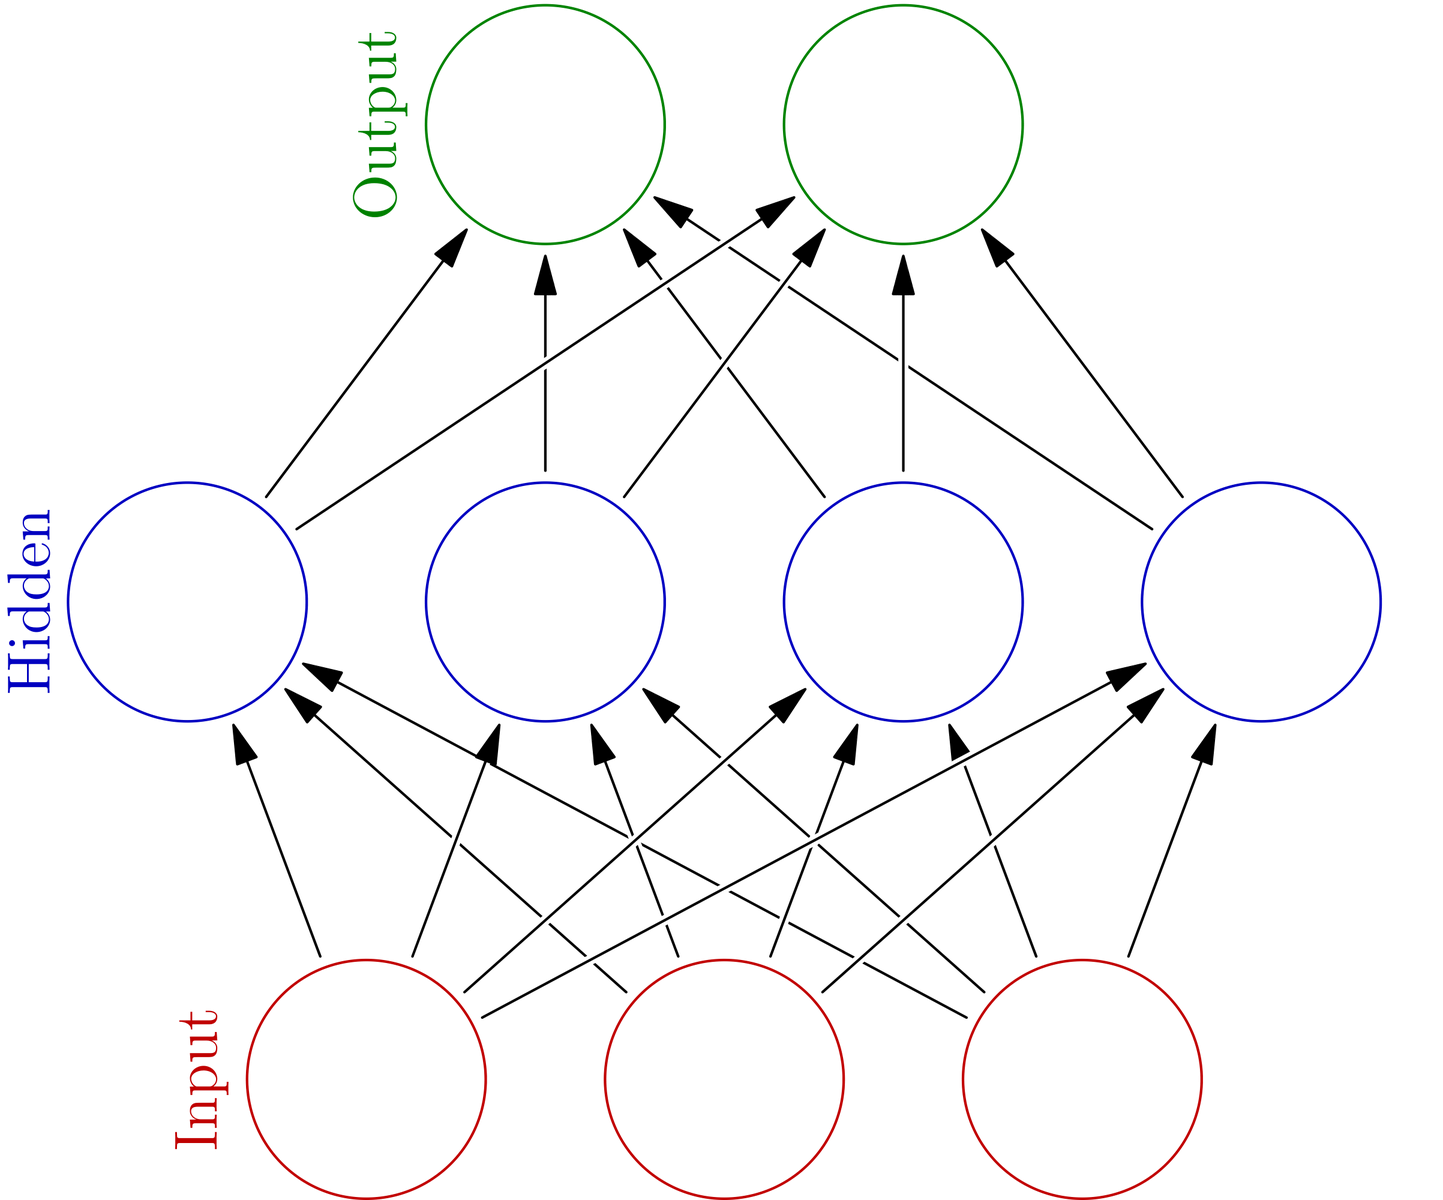
\includegraphics[scale = 0.2]{imm/colored_neural_network-1200x1443.png}
    \label{fig:my_label}
\end{figure}

Quindi fissata una mappa $f$ tra input e output, sulla base degli stimoli $x_k$, la rete cambia i pesi in modo che dopo un numero finito di passi $s$ si abbia l'output $y_k$ tale che $f(x_k)=y_k,\forall\,k>s$ (almeno approssimativamente). Per la modifica bisogna minimizzare un \textbf{criterio di discrepanza} tra risposta della rete e risposta desiderata.\\

%% io non ho aggiunto l'esempio, me lo sono solamente guardato

Viene aumentata la potenza rispetto al percettrone, permettendo una classificazione \textbf{altamente non lineare}.\\ 

\subsubsection{Unità sigmoidi}
Si hanno quindi $u_1,\ldots, u_n$ neuroni divisi in: \begin{itemize} 
    \item unità di input 
    \item unità nascoste 
    \item unità di output 
\end{itemize} 
Si hanno inoltre: 
    \begin{itemize} 
    \item pesi $w_jj$ per ogni coppia che voglio connettere 
    \item stati di attivazione $s_j\in \mathbb{R}$ 
    \item input netto a $u_j$: $n_i=\displaystyle\sum_{i=0}^n w_{ij}\cdot s_i$ \item funzione di transizione sigmoide: $s_j(t+1)=\displaystyle \frac{1}{1+e^{-n_i(t)}}$ 
\end{itemize}

Lo stato di uscita è determinato da una serie di strati profondi. Dato un input $x$, un output target $t$ e un output effettivo $y$. Si consideri la forma quadratica: $E=\frac{1}{2}\sum_j(t_j-y_j)^2$ che dipende anche dagli strati nascosti. 
I pesi vengono modificati usando la seguente formula: $\displaystyle\Delta w_{ij}=-\eta\cdot\frac{\partial E}{\partial w_{ij}}$ poiché: \\ $\displaystyle\frac{\partial E}{\partial w_{ij}}= \frac{\partial E}{\partial n_{j}}\cdot \frac{\partial n_j}{\partial w_{ij}}= \frac{\partial E}{\partial n_{j}}\cdot s_j=(def)-\delta_j\cdot s_j$, dobbiamo determinare  $\displaystyle\delta_j=-\frac{\partial E}{\partial n_{j}}$

Per poter arrivare a determinare quanto ci interessa, dobbiamo utilizzare l'\textbf{algoritmo di retropropagazione}, a sua volta quest'ultimo che si divide in 5 passi.

\subsubsection{Algoritmo di retropropagazione}
I passi da cui è composto sono i seguenti:
\begin{enumerate}
    \item \textbf{Input}: al neurone di input $u_j$ viene assegnato lo stato $x_j$
    \item \textbf{Propagazione}: si calcola lo stato dei neuroni nascosti o di output $u_j$: $s_j=f_j(n_j)$
    \item \textbf{Confronto}: per ogni neurone di output $u_j$, noto l’output atteso $t_j$, si calcola:  $\delta_j=f_j(n_j)\cdot(t_j-y_j))$
    \item \textbf{retropropagazione dell’errore}: per ogni neurone nascosto $u_j$, si calcola: $\displaystyle\delta_j=f_j(n_j)\cdot\left(\sum_h w_{jh}\cdot \delta_h\right)$
    \item \textbf{aggiornamento dei pesi}: si ha: $\displaystyle w_{ij}=w_{ij}+\eta\cdot \delta_i\cdot s_j$
\end{enumerate}
Nelle prime due fasi viene calcolato principalmente l'output, nel terzo verifico l'errore e nelle ultime due aggiorno i pesi.

\begin{algorithm}[H]
    \SetAlgoLined
    \textnormal{Inizializzo ogni} $w_i$ \textnormal{ con un piccolo valore casuale} \\
    \While{\textnormal{Fino al raggiungimento della condizione di terminazione}}{
        \For{\textnormal{ogni input } $\langle x_1, \ldots x_n),t \rangle$}{
            Immetti $(x_1, \dots ,x_n)$ nella rete e calcola l'output $y_k$ \\
            \For{\textnormal{Per ogni unità di output } k}{
                $\delta_k=y_k\cdot(1-y_k)\cdot(t_k-y_k)$ \\        
            }
            \For{\textnormal{Per ogni unità nascosta } h}{
                $\delta_h=y_h\cdot(1-y_h)\cdot\sum_k w_{hk}\delta_k$ \\        
            }
            \For{\textnormal{Per ogni peso } $w_{i,j}$}{
            $w_{ij}=w_{ij}+\Delta w_{ij},\mbox{ con } \Delta w_{ij}=\eta\cdot\delta_j\cdot x_{ij}$
            }
        }
   }
   \caption{Algoritmo di retropropagazione}
\end{algorithm}

Questo algoritmo, che ha una discesa lungo il gradiente rispeto all'intero vettore dei pesi, si generalizza facilmente a grafi orientati arbitrari.\\ Si trova però un \textbf{minimo locale}, non necessariamente \textbf{globale}, e spesso include \textbf{termini di momento} per cambiare la formula dell'aggiornamento dei pesi del tipo: 
$\Delta w_{ij}(n)=\eta\cdot \delta_j\cdot x_{ij}+\alpha\Delta w_{ij}(n-1)$ in modo da avere una sorta di \textit{inerzia} per la variazione dei pesi.\\ 
Ci sono comunque modelli per uscire dai minimi locali.\\ 
Si minimizzano gli errori sugli esempi di training, ma si rischia l'\textbf{overfitting}.\\ 
Tutti questi fattori comportano un addestramento lento ma dopo l'addestramento si ha una rete veloce.\\

L'algoritmo ha diversi limiti:
\begin{itemize}
  \item mancanza di teoremi generali di convergenza
  \item può portare in minimi locali di $E$ 
  \item difficoltà per la scelta dei parametri 
  \item scarsa capacità di generalizzazione 
\end{itemize}
Si possono apportare diverse modifiche per apportare qualche miglioria al modello tramite:
\begin{itemize}
  \item un tasso di apprendimento adattivo: $\eta=g(\nabla E)$
  \item termine di momento $\Delta w_{ij}(n)=\eta\cdot \delta_j\cdot x_{ij}+\alpha\Delta w_{ij}(n-1)$
  \item range degli stati da –1 a 1 
  \item deviazioni dalla discesa più ripida 
  \item variazioni nell'architettura (numero di strati nascosti)
  \item inserimento di connessioni all'indietro
\end{itemize}
% salta le slide a caso
\textit{Le reti \textbf{feedforward} sono state usate in progetti di guida autonoma come \textbf{ALVINN}.}\\
%salta altre slide e non so se bisogna aggiungere altro

\section{Support Vector Machine}
Per il percettrone semplice veniva usato un algoritmo di apprendimento per fargli imparare solo funzioni di separazione lineari, e mentre il percettrone multistrato poteva imparare funzioni di separazione non lineari complesse, ma con difficoltà di addestramento avendo molti minimi locali e tanti pesi, le \textbf{SVM} funzionano usando un algoritmo di apprendimento efficiente per imparare funzioni di separazione non lineari complesse. 

Viene quindi ripreso comunque il concetto di \textit{separazione lineare} ma con una scelta efficiente dell'iperpiano. Quando si il SVM, si usa un metodo che prende tutte le istanze in input, esegue un calcolo immediato di quelle che è un set di dati buono. Si trova così il \textbf{miglior iperpiano separatore}, per classificare un insieme di punti linearmente separabili, trovando un vettore di pesi $W$ per separare bene le istanze. 
Si usa la cosiddetto \textbf{teoria statistica dell’apprendimento} che dice che tra tutti gli iperpiani che possiamo usare per separare due classi si sceglie quello che probabilmente sarà in grado di etichettare meglio nel futuro. Con le SVM inoltre si vedrà come si comporta l'iperpiano sugli esempi non visti, generati sempre da una $f$, ma che non abbiamo potuto considerato per poter produrre il vettore, o i vettori, di peso.  
Per scegliere il miglior iperpiano viene utilizzato con l'intuizione. L'intuizione è quella di prendere un iperpiano ottimo rispetto alla misura della distanza minima che si ha tra gli esempi e l'iperpiano stesso.
Quello che si fa è guardare tutti i punti del mio training set e cercare di scoprire a quale degli iperpiani si avvicinano di più. L'obbietivo sembra essere inserire l'iperpiano in mezzo ai punti (quindi è la riga che divide in modo perfetto, con le stesse distanze dai punti vicini, l'iperpiano positivo e negativo), in modo che intorno ad esso ci sia massima ampiezza. Tale ampiezza è detta margine (volendo che sia massima la distanza minima tra tutti i punti). SVM usa questa teoria per trovare l'iperpiano migliore in base a questi calcoli probabilistici.  \\
Notiamo facilmente che non si parla quindi più di neuroni. \\

Se riuscissimo a separare i dati con un largo margine avremmo ragione di credere che (assunto che i punti siano generati sempre dalla stessa “regola” ) il classificatore (ovvero l'iperpiano stesso) sia “più robusto” tanto da avere una migliore generalizzazione. Il nostro classificatore (iperpiano o $f$) divide correttamente i punti su cui è stato addestrato. \\
Quando arriva quindi un nuovo punto, generato con la stessa regola degli altri, sarà sicuramente classificato correttamente, una volta scelto l'iperpiano.\\ 
Ci serve quindi la separabilità delle istanze, serve quindi che la funzione generatrice sia linearmente separabile. \\
La probabilità di avere un buon comportamento su istanze future è valutabile rispetto a una classe di funzioni segrete, generatrici delle istanze, che sia ben nota. Se la classe di separazione fosse non linearmente separabile quello che il mio sistema è molto limitato. 
\subsection{Vapnik-Cervonenkis - VC}
Con la teoria statistica dell'apprendimento si dimostra che più allarghiamo il margine meglio l’iperpiano generalizza, raggiungendo la dimensione di Vapnik-Cervonenkis (VC).\\ Prese tutte le funzioni che generano il training set si produce la VC che esprime quanto è difficile sbagliare sulle ipotesi future in base alla scelta dell'iperpiano.\\

Dobbiamo quindi scrivere un algoritmo per trovare l'iperpiano di separazione di massimo margine. In input si hanno le istanze etichettate e in output un vettore (è un numero) che identifica l'iperpiano.\\ 
Viene usata una notazione matematica, dove supponiamo di avere un insieme di punti di training: \\ $S = \{(x_1,y_1), (x_2,y_2),\ldots, (x_n,y_n)\}$. Ad ogni $x_i$ (vettore) è associata la rispettiva classe di appartenenza $y_i$ (con etichetta binaria non booleana), infatti $y_i \in \{-1,\ +1\}$.\\
I punti sono linearmente separabili (inoltre dalle formule si nota che l'iperpiano separa positivi e negativi)
\[
  \begin{cases}
    \langle w,x_i\rangle + b >0 &\mbox{ se }y_i=+1\\
    \langle w,x_i\rangle + b <0 &\mbox{ se }y_i=-1\\
  \end{cases}
\] \\
Ma questo lo possiamo scrivere in modo equivalente usando un solo vincolo: $y_1 \cdot \langle w,x_i\rangle + b >0 \quad i= 1,\dots, n$.\\ 
Come risultato del nostro apprendimento cerchiamo i valori $w$ e $b$. Si ha che $w$ mi dirà quanto è inclinato il piano mentre $b$ è la distanza tra l'origine e il piano. Queste due variabili identificano i vari iperpiani possibili tra cui cercare il migliore ovvero quello che separa meglio punti positivi e negativi.\\ 
Noi cerchiamo quindi tra gli iperpiani separatori ($w$, $b$), oppure tra le funzioni di decisione lineari associate, espresse nella forma $h_{w,b}(x) = sgn(\langle w,x \rangle + b)$, il migliore iperpiano, o la migliore funzione di decisione, che meglio separa i punti negativi da quelli positivi. \\

Sia $d_-$ e $d_+$ le distanze tra l’iperpiano separatore e il punto positivo e negativo più vicino definiamo il:
\begin{itemize}
    \item \textbf{margine funzionale} di un punto $(x_i,y_i)$ rispetto all’iperpiano $(w,b)$: $\hat{\gamma} = y_i(\langle w, x \rangle +b)$\\ Il margine funzionale dell'iperpiano rispetto al training set $S$ è il valore minimo:$\hat \rho = \displaystyle \min_{i = 1, \dots, n} \hat{\gamma}_i$.
    Se il punto $x_i$ è tale che $y_i = +1$ ($y_i = -1$), affinché il margine funzionale sia grande, è necessario che la quantità $\langle w, x_i \rangle$ abbia un valore positivo (negativo).\\
    Per ogni istanza $i$, se $\hat{\gamma}_i > 0$, la classificazione è corretta, ovvero le classi sono linearmente separabili e l’iperpiano $(w, b)$ le separa effettivamente.\\
    Un ampio margine funzionale dà speranza sulla qualità della predizione ma bisogna tenere conto anche altri aspetti.
    Il margine funzionale non è invariante rispetto ad un iperpiano riscalato, ovvero per come è stato impostato il classificatore $f$, se si scala l’iperpiano $(w,b) \to (cw, cb)$:
    \begin{itemize}
        \item si ottiene lo stesso iperpiano, ovvero lo stesso luogo dei punti
        \item si ottiene la stessa funzione di decisione, eventualmente con segno invertito se $c$ è negativo
        \item il margine funzionale viene moltiplicato per $c$ e non è quindi possibile usarlo come distanza di un punto dall’iperpiano perché non è invariante rispetto alla scala. 
    \end{itemize}
    \item \textbf{margine geometrico} dell’iperpiano rispetto al training set $S$: $\rho = \displaystyle \min_{i = 1, \dots, n}\gamma_i$.\\
    Distanza dall’iperpiano a un punto $x$: $d = \displaystyle \frac{\displaystyle  \sum_{i=1}^n w_i x_i + b}{|| w ||} = \displaystyle  \frac{\langle w \cdot x_i \rangle + b}{|| w||}$.\\
    Margine geometrico di un punto $(x_i, y_i)$ rispetto all’iperpiano $(w,b)$: $\gamma_i = \displaystyle \frac{y_i(\langle w, x_i \rangle + b)}{||w||}$. \\
    Per ogni istanza $i$, se $\gamma_i > 0$, la classificazione è corretta, come per il margine funzionale. Dato un punto positivo (negativo) il margine geometrico rappresenta la sua distanza geometrica dall’iperpiano in $R^n$.

  Il margine geometrico è invariante rispetto alla scala di w. \\
  Grazie a tale invarianza, si può riscalare l’iperpiano senza cambiare nulla (il margine non varia). Se si pone $||w|| = 1$, si riscala l’iperpiano $(w,b) \to (\displaystyle \frac{w}{||w||}, \frac{b}{||w||})$, andando a considerare l’iperpiano $(\displaystyle \frac{w}{||w||}, \frac{b}{||w||})$ con vettore pesi $\displaystyle \frac{w}{||w||}$ di norma unitaria.
\end{itemize}

\bigskip

Un iperpiano è detto \textbf{canonico}, se $\displaystyle \min_{i = 1, \dots, n}|\langle w,x_i \rangle+ b| = 1$. \\
In altri termini, per un iperpiano canonico il margine funzionale è $1$ e il margine geometrico è $\displaystyle \frac{1}{||w||}$. 
Se $||w|| = 1$, il margine funzionale è uguale al margine geometrico, infatti: $\gamma_i = \displaystyle \frac{y_i(\langle w, x_i \rangle + b)}{||w||}$ e $\hat \gamma_i = y_i (\langle w,x \rangle + b)$.\\

Relazione tra margine funzionale e geometrico: $\gamma = \displaystyle \frac{\hat \gamma}{||w||}$.\\
Per quanto detto, sembra naturale il voler cercare di estendere quanto possibile il margine geometrico, risolvendo un problema di ottimo del tipo:  $\max f(x)$ tale che $g(x) \leq 0, \;  h(x)=0$. Non sempre esiste una soluzione e, se esiste, difficilmente la si riesce a trovare per via analitica; a volte si può approssimare con metodi iterativi.

Per assicurarsi che tutti punti (sia positivi che negativi) cadano al di fuori del margine, dato un $\gamma$, per ogni punto $i$, si vuole che $\displaystyle \frac{y_i(\langle w, x_i \rangle + b)}{||w||} \geq \gamma$. Il problema di ottimo diventa quindi: 
$$\max (\gamma) \mbox{ tale che } y_i(\langle w, x_i \rangle + b) \geq \gamma, \;  ||w||=1$$ 

Un problema così formulato è di difficile soluzione perché presenta un vincolo non convesso. Riformulandolo, in modo da scrivere il margine geometrico come $\gamma = \displaystyle \frac{\hat \gamma}{||w||}$, diventa:  $\max \displaystyle \frac{\hat\gamma}{||w||}$ tale che $y_i(\langle w, x_i \rangle + b) \geq \hat \gamma$. \\
Sussiste ancora un problema, ovvero il fatto che l’obiettivo sia non convesso. Dal momento che si può scalare l’iperpiano senza cambiare nulla (invarianza), è possibile riscalare $(w,b)$ in modo che il margine funzionale sia $1$ (ottenendo un iperpiano canonico): $\max \displaystyle \frac{1}{||w||}$ tale che $y_i(\langle w, x_i \rangle + b) \geq 1$\\ 

Rendere massimo $\displaystyle \frac{1}{||w||}$ equivale a rendere minimo $\displaystyle \frac{1}{2}||w||^2$, quindi: 
$$\min \tau(w) = \displaystyle \frac{1}{2}||w||^2 \mbox{ tale che } y_i(\langle w, x_i \rangle + b) \geq 1, \mbox{ con } i = 1, \dots, n$$

e si ha che:$w=\displaystyle \sum_{i\in Q}\alpha_i \cdot x_i$. \\
Quest’ultima forma è quella su cui si lavora. Si può dimostrare che esiste una sola soluzione al problema, ovvero che esiste un unico iperpiano di massimo margine.
Due motivi che supportano il metodo delle SVM: la capacità dell’iperpiano di effettuare una separazione di massimo margine e l’esistenza di un’unica soluzione al problema. La soluzione al problema è scritta in termini di un sottoinsieme di esempi del training set (noto come vettori di supporto) che giacciono sul margine dell’iperpiano, prendendo una somma pesata dei contenuti dei vettori.\\

Per classificare un nuovo elemento (vettore)$x$ ci interessa il segno di $\langle w,x\rangle+b$ che possiamo scrivere come:

$$sgn(\langle w,x\rangle+b)=sgn\displaystyle \left(\Big\langle\sum_{i\in Q}\alpha_i\cdot  x_i,x\Big\rangle +b\right)=sgn\left(\sum_{i\in Q}\alpha_i\langle x_i,x\rangle +b\right)$$
Quindi la funzione di decisione associata alla soluzione può essere scritta in termini del prodotto interno tra i vettori di supporto (\textit{support vector}) $x_i$ e il vettore da classificare $x$.$\alpha$ viene elaborato dai vettori di supporto ma non verrà ora trattato.\\

Passiamo quindi oltre alla sola separabilità lineare.\\

Si usa lo stesso approccio, rivedendo la formulazione, tramite i \textbf{metodi kernel}. Si cerca di mappare lo spazio di input in un nuovo spazio, (in generale di dimensione maggiore), in cui i punti siano linearmente separabili, per classificare mediante superfici non lineari.\\

Dobbiamo trovare una funzione: $\Phi:\mathbb{R}^n\to \mathbb{R}^m,\mbox{con }m>n$ che mappi i dati iniziali non linearmente separabili in uno spazio di dimensione
superiore in cui siano linearmente separabili.\\
In questo nuovo spazio la funzione di decisione che classifica l'input $x$ è: $sgn\left(\displaystyle \sum_{i\in Q}\alpha_i\langle \Phi(x_i),\Phi(x)\rangle+b\right)$. \\
Il calcolo delle immagini $\Phi(x_i)$ è generalmente computazionalmente pesante ma è semplificato nel caso di \textbf{funzioni kernel}.
\subsection{Funzione kernel}
Data una trasformazione $\Phi:\mathbb{R}^n\to \mathbb{R}^m$ una \textbf{funzione kernel} è una mappa: \\
$$K:\mathbb{R}^n\times \mathbb{R}^n\to \mathbb{R}\mbox{ in modo tale che }K(x,y)=\Phi(x)\cdot \Phi(y)$$
Il kernel ha una particolarità, il \textbf{kernel trick}: che consiste nel computare il prodotto interno delle trasformare di due vettori $x$ e $y$, tramite $\Phi$, senza computare le trasformate, semplificando il calcolo della funzione di decisione:$$sgn\left(\displaystyle \sum_{i\in Q}\alpha_i\langle \Phi(x_i) , \Phi(x) \rangle + b \right)$$ sostituendo $\Phi(x_i)\cdot\Phi(x)$ con $K(x_i,x)$, ottenendo: $sgn\left(\sum_{i\in Q}\alpha_i\cdot K(x_i,x)+b\right)$  con: $K(x,y)=\langle \Phi(x) , \Phi(y) \rangle$\\
Non si cercano tutte le possibili trasformazioni ma solo alcune.

%###qui fa un esempio, l'ho seguito ma non mi sembrava impo da scrivere

Si hanno alcune proprietà in riferimento alle funzioni kernel:
\begin{itemize}
  \item se i dati sono mappati in uno spazio di dimensioni sufficientemente elevate, saranno quasi sempre linearmente separabili
  \item quattro dimensioni sono sufficienti per separare linearmente un cerchio in qualsiasi punto del piano
  \item cinque dimensioni sono sufficienti per separare linearmente qualsiasi ellisse
  \item se abbiamo $N$ esempi sono quasi sempre separabili in spazi di dimensioni $N-1$ o più
  \item rappresentano un modo per applicare le SVM in modo efficiente in spazi di dimensione molto alta (o infinita): $$
    K(x,y) = \langle \Phi(x) , \Phi(y) \rangle, \mbox{ con } \Phi: \mathbb{R}^n \to \mathbb{R}^m
  $$
  \item calcolare $K(x,y)$ può essere molto economico anche se $\Phi(x)$ è molto costoso, ad esempio con vettori di dimensione elevata, in tali casi (che vanno dimostrati), si addestrano le SVM nello spazio di dimensionalità maggiore senza mai dover trovare o rappresentare esplicitamente i vettori $\Phi(x)$
\end{itemize}

Vediamo due teoremi:
\begin{itemize}
    \item Un kernel definisce una matrice [$K_{ij}$] che è simmetrica e definita positiva
    \item Ogni matrice simmetrica e definita positiva è un kernel [Teorema di Mercer]
\end{itemize}

\section{Lezione 7 - SVM}
SVM può essere applicato a problemi non binari tramite il \textbf{one vs rest}, avendo separazioni non più solo tra esempi positivi e negativi ma anche tra più classi, ovvero più gruppi di punti linearmente separabili.\\
In caso di SVM multiclasse è possibile trasformare il problema di partenza in una serie di sottoproblemi binari derivati (isolando una classe per volta considerata positiva, da tutto il resto dei dati considerato negativo,  \textbf{one vs rest}) sui quali applicare SVM e ricombinare con una qualche logica di classificazione i vari risultati ottenuti.\\
In input si prende un learner $L$ (ovvero un algoritmo di addestramento per la classificazione binaria), un set di $K$ esempi $\langle x_i, y_i \rangle$ con $y_i$ label associata all’istanza $x_i$.\\
In output si ottiene una lista di classificatori $f_k$ con $k=1,\ldots K$.
Per quanto riguarda la procedura quindi, $\forall k\in \{1\ldots K\}$ si costruisce un nuovo vettore di label $z$ tale che: 
$$\begin{cases}
    z_i=y_i&\mbox{ se } y_i=k\\
    z_i=0&\mbox{ altrimenti}
\end{cases}$$ e si applica poi $L$ a $(X,z)$ per ottenere $f_k$.\\
Quindi prendere decisioni significa applicare tutti i classificatori ad un nuovo esempio e prevedere l’etichetta $k$ per la quale il classificatore corrispondente riporta il punteggio di confidenza più alto, una sorta di peso per la classificazione dell’esempio.

Questa euristica soffre di diversi problemi:
\begin{itemize}
    \item la scala dei valori di confidenza può differire tra vari classificatori binari.
    \item anche se la distribuzione in classe è bilanciata nel training set, i learner per la classificazione binaria vedono distribuzioni sbilanciate perché tipicamente l’insieme di negativi che vedono è molto più grande dell’insieme di positivi.
\end{itemize}

Un’alternativa è il \textbf{one vs one} che prende le varie classi e produce sistemi di SVM tra coppie di classi. \\
Il problema di questa alternativa è che la quantità di problemi derivati esplode in modo quadratico.\\
Si ha il train di $$\frac{K\cdot (K-1)}{2}$$ classificatori binari per un problema a $K$ classi, ognuno dei quali riceve i campioni di un paio di classi dal training set originale che deve imparare a distinguere.
In fase di predizione tutti i $\frac{K\cdot (K-1)}{2}$ classificatori sono applicati al nuovo esempio e la classe che con il più alto numero di predizioni positive viene usata come previsione per il classificatore combinato. 
Anche questa tecnica soffre di ambiguità in quanto alcune regioni del suo spazio di input possono ricevere lo stesso numero di voti.
\section{Apprendimento Bayesano}
Nell'ambito Bayesano si cambia l'approccio avendo la valutazione di ipotesi in base alla loro probabilità. Si studia la probabilità rispetto ai dati e rispetto
alle conoscenze pregresse. Non troviamo un'ipotesi che combacia ma che è probabile.\\

Bisogna studiare come scegliere le ipotesi, usando risultati noti del calcolo probabilistico e quindi come funziona l'apprendimento. Useremo le nozioni di probabilità e probabilità condizionata, oltre ovviamente alla \textbf{regola di Bayes}. Il meglio è definito quindi tramite probabilità.\\ 

Si assume quindi che le quantità di interesse siano governate da distribuzioni di probabilità e che la decisione migliore può essere presa ragionando su tali distribuzioni e sull'insieme di dati di training. L'apprendimento Bayesano è importante per due ragioni principali: 
\begin{enumerate}
  \item si ha una manipolazione esplicita delle probabilità rispetto ad altri approcci pratici di alcuni tipi di problemi di apprendimento (infatti si hanno spesso paragoni con gli alberi decisionali e con le reti neurali)
  \item fornisce una prospettiva utile per comprendere metodi di apprendimento che non manipolano effettivamente le probabilità
\end{enumerate}

Andando a considerare quelle che sono le caratteristiche del Bayesiano, si ha che ogni esempio di training osservato può aumentare o diminuire, in modo incrementale, la stima di probabilità relativa alla correttezza di un'ipotesi. Inoltre, come già anticipato, la conoscenza pregressa può essere combinata con i dati osservati per determinare la probabilità finale delle varie ipotesi. \\

Si ha inoltre che le varie ipotesi possono effettuare predizioni probabilistiche, le nuove istanze possono essere classificate combinando le predizioni delle ipotesi, che sono pesate attraverso la loro stessa probabilità. Con il metodo Bayesano si ottiene quindi uno standard per prendere decisioni ottimali attraverso il quale, altre misure pratiche, possono essere misurate. \\

Si hanno però alcune difficoltà legate all'apprendimento Bayesano:
\begin{itemize}
  \item si necessita avere la conoscenza di varie probabilità
  \item si hanno costi computazionali non indifferenti
\end{itemize}

\subsection{Teorema di Bayes}
Ponendo l'attenzione nel macchine learning dove si è interessati a trovare la migliore ipotesi $h$, presente in uno spazio delle ipotesi $H$, una volta eseguito l'addestramento su un training data $D$.  Il teormea di Bayes(o se vogliamo nell'apprendimento Bayesano) si ragiona in termini differenti, si ha che la miglior ipotesi altro non è che la più probabile. Per quanto riguarda la probabilità, la possiamo calcolare basandoci: sulla probabilità conosciuta a priori, sulla distribuzione dei dati che vado a osservare o dai dati stessi. 

\begin{teorema}{Teorema di Bayes}{}
    Il teorema enuncia che: \[P(h|D)=\frac{P(D|h)P(h)}{P(D)}\]
    Avendo:
    \begin{itemize}
        \item $P(h)$:   probabilità conosciuta a priori di $h$. Tale probabilità riflette qualsiasi conoscenza di base sulla possibilità che $h$ sia corretta  
        \item $P(D)$:   probabilità conosciuta a priori di $D$, ovvero la probabilità che $D$ sia osservato
        \item $P(D|h)$: probabilità di osservare $D$ in presenza dell'ipotesi $h$
        \item $P(h|D)$: probabilità a posteriori di $h$. Tale probabilità riflette la confidenza che $h$ sia valida dopo che $D$ è stato osservato
    \end{itemize}
\end{teorema}

Cercando di semplificare l'approccio computazione, evitando quindi di considerare tutte le $D$ e tutte le $h$, esistono altre soluzioni. 
In molti scenari di apprendimento, il learner considera un insieme di ipotesi candidate $H$ ed è interessato a trovare l'ipotesi più probabile $h\in H$, in base ai dati osservati in $D$.\\
Definiamo le ipotesi \textit{ maximum a posteriori (MAP)} ogni ipotesi massimamente probabile e la indichiamo:
    \begin{equation*}
        \begin{split}
            h_{MAP}&=\operatorname*{argmax}_{h\in H}P(h|D)\\
            & = \operatorname*{argmax}_{h\in H}\frac{P(D|h)P(h)}{P(D)}\\
            & = \operatorname*{argmax}_{h\in H}P(D|h)P(h)
        \end{split}
    \end{equation*}
L'ultimo passaggio viene eseguendo tenendo nota che $P(D)$ può essere cancellato in quanto costante e indipendente da $h$.\\

Spesso si assume anche che ogni ipotesi è a priori equiprobabile e quindi possiamo semplificare ulteriormente i conti. Dato che $P(D|h)$ viene spesso chiamata \textbf{likehood (\textit{probabilità})} di $D$ data $h$ viene definita ipotesi\textbf{ maximum likehood (ML)} ogni ipotesi che massimizza $P(D|h)$ descrita come segue: \[h_{ML}=\operatorname*{argmax}_{h\in H}P(D|h)\]
potendo quindi trascurare $P(h)$ in quanto costante e uguale $\forall\,h\in H$\\

Si può usare il teorema di Bayes per specificare un algoritmo di apprendimento molto semplice detto \textbf{algoritmo Brute-Force MAP LEARNING} che si articola
in 2 step:
\begin{enumerate}
  \item $\forall\,h\in H$ calcolo la probabilità a posteriori tramite il teorema di Bayes: \[P(h|D)=\frac{P(D|h)P(h)}{P(D)}\]
  \item restituisco l'ipotesi $h_{MAP}$ con la più alta probabilità a posteriori: \[h_{MAP}=\operatorname*{argmax}_{h\in H}P(h|D)\]
\end{enumerate}
Per specificare un problema di apprendimento per l'algoritmo bisogna specificare i valori di $P(h)$ e $P(D|h)$, e in base a questo dobbiamo fare alcune assunzioni:
\begin{itemize}
  \item il training set deve essere privo di rumore, avendo: $d_i=c(x_i)$
  \item il target concept deve essere contenuto nello spazio delle ipotesi $H$, dettagliatamente si dirò che: 
  $\exists h\in H \ : \  \forall\, x\in X$ si ottiene che $ h(x)=c(x)$
  \item devo assumere che le ipotesi siano equiprobabili e quindi: $P(h)=\displaystyle \frac{1}{|H|}\quad \forall h\in H$
  riducendoci ad avere:
  \[P(D|h)=
    \begin{cases}
      1&\mbox{se } d_i=h(x_ i),\,\,\,\forall\,d_i\in D\\
      0&\mbox{altrimenti}
    \end{cases}
  \]
\end{itemize}

Ora che abbiamo completamente definito l'algoritmo di apprendimento, in un primo passaggio dobbiamo determinare le probabilità dei nostri $P(h|D)$:
\begin{itemize}
   \item $h$ è inconsistente con $D$, avendo quindi: $P(h|D)=\displaystyle\frac{0\cdot P(h)}{P(D)}=0$
  \item $h$ è consistente con $D$, avendo quindi: $\displaystyle P(h|D)=\frac{1\cdot \frac{1}{|H|}}{P(D)} = \frac{1\cdot \frac{1}{|H|}}{\frac{|V\ S_{H,D}|}{|H|}}=\frac{1}{|V\ S_{H,D}|}$ 
\end{itemize}
Questa analisi implica il fatto che, in base a queste assunzioni, ogni iptotesi consistente è una ipotesi $MAP$, questo perché $\forall h$ che è consistente, $\displaystyle P(h|D) = \frac{1}{|V\ S_{H,D}|}$

\begin{figure}[H]
    \centering
    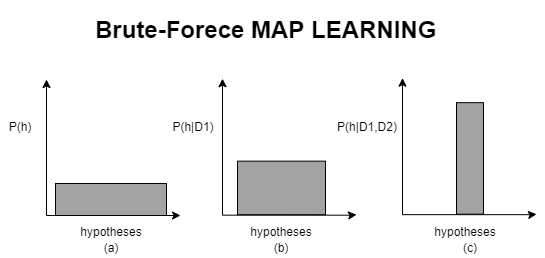
\includegraphics[scale = 0.7]{imm/foto_map.png}
\end{figure}
Dove (a) corrisponde a dire che tute le ipotesi hanno la stessa probabilità, invece (b)+(c) si ha che mentre i dati di addestramento si accumulano, la probabilità a posteriori delle ipotesi inconsistenti diventa zero mentre la probabilità totale che si somma a 1 è condivisa in maniera equa tra le ipotesi consistenti rimanenti.\\

Si ha che ogni learner consistente ha in output ipotesi MAP, se si assume a priori la distribuzione uniforme delle probabilità su $H$ dati di training deterministici e privi di rumore.\\

Riprendendo l'algoritmo find-S si ha che: 
\begin{itemize} 
    \item ha in output ipotesi consistenti e quindi ipotesi MAP sotto la distribuzione di probabilità $P(h)$ e $P(D|h)$ 
    \item $\forall\,P(h)$ che favorisce le ipotesi più specifiche, find-S trova appunto le ipotesi MAP 
\end{itemize} 

A riprova che il metodo Bayesano è un modo per caratterizzare il comportamento degli algoritmi di apprendimento, identificando le distribuzione di probabilità $P(h)$ e $P(D|h)$ in base alle quali l'output è l'ipotesi ottimale, è possibile caratterizzare le ipotesi implicite dell'algoritmo ovvero il \textbf{bias induttivo}.\\

Si introduce ora il problema di apprendere funzioni target a valori continui (coime reti neurali o regressione lineare). Si ha che in base a determinate assunzioni, qualsiasi algoritmo di apprendimento che minimizzi l'errore quadratico (scarto quadratico??) tra l'ipotesi di output e i dati di addestramento, produrrà un'ipotesi ML.\\
Si imposta il problema come segue:
\begin{itemize}
    \item $\forall\,h\in H$,  $h:X\to\Re$, avendo esempi della forma $\langle x_i, d_i\rangle$
    \item la funzione target è definita come $f:X\to\Re$
    \item si hanno $m$ esempi di training dove il valore target di ogni esempio è sporcato dal rumore casuale secondo una distribuzione di probabilità normale con media nulla, avendo $d_i=f(x_i)+e_i$
\end{itemize}

Avendo quindi che $h_{ML}=\operatorname*{argmax}_{h\in H}P(D|h)$ e che gli eventi di training vengono assunti come indipendenti si ha che: $$h_{ML}=\operatorname*{argmax}_{h\in H}\prod_{i=1}^mP(d_i|h)$$ \\

Dato quindi l'errore ($e_i$) distribuito normalmente con media zero e varianza sconosciuta $\sigma^2$ si ha che anche ogni $d_i$ deve seguire la stessa distribuzione attorno al valore target $f(x_i)$. Poiché stiamo scrivendo l'espressione per $P(D|h)$, assumiamo che $h$ sia la descrizione corretta per $f$, quindi: $\mu=f(x_i)=h(x_i)$, e avendo quindi, per la distribuzione normale: 
\[h_{ML}=\operatorname*{argmax}_{h\in H} \prod_{i=1}^m\frac{1}{\sqrt{2\pi\sigma^2}} e^{-\frac{1}{2\sigma^2}(d_i-h(x_i))^2}\]
È comune massimizzare il logaritmo meno complicato, il che è ragionevole per via della monotonia di questa funzione, ottenendo:
\[h_{ML}=\operatorname*{argmax}_{h\in H}\sum_{i=1}^m\ln{\frac{1}{\sqrt{2\pi\sigma^2}}} -\frac{1}{2\sigma^2}(d_i-h(x_i))^2\]
ma il primo termine è costante e indipendente da $h$ e quindi può non essere considerato:
\[h_{ML}=\operatorname*{argmax}_{h\in H}\sum_{i=1}^m -\frac{1}{2\sigma^2}(d_i-h(x_i))^2\]
Sapendo che massimizzare questo termine negativo equivale a ridurre al minimo il termine positivo corrispondente:
\[h_{ML}=\operatorname*{argmin}_{h\in H}\sum_{i=1}^m \frac{1}{2\sigma^2}(d_i-h(x_i))^2\]
e avendo che anche tutte le costanti sono indipendenti da $h$ e quindi possono essere rimosse:
\[h_{ML}=\operatorname*{argmin}_{h\in H}\sum_{i=1}^m (d_i-h(x_i))^2\]
trovando che $h_{ML}$ è ciò che minimizza gli errori quadratici. \\

Si specifica la scelta della normale in quanto:
\begin{itemize}
  \item buona approssimazione di molti tipi di rumore nei sistemi fisici 
  \item il Teorema del Limite Centrale mostra che la somma di un numero sufficientemente grande di variabili casuali indipendenti e identicamente distribuite obbedisce a una distribuzione Normale
\end{itemize}

Si considera solo il rumore sul valore del target e non sugli attributi che descrivono le istanze stesse.\\ 
Anche in questo caso si usa il Rasoio di Occam, scegliendo di usare il principio \textbf{Minimum Description Length (\textit{MDL})}, scegliendo la spiegazione più breve per i dati osservati.\\

%% qui dice che riprenderà una slide

\subsection{Classificatore Bayesano ottimale per la classificazione}
Ci si chiede quindi qual è la classificazione più probabile della nuova istanza secondo i dati di training.\\
Applicare solamente $h_{MAP}$ non basta, questo perché non risulta la migliore situazione in alcune situazioni. \\

%%%Solo xk poi lo usa come concetto:
Sia $H = \{h_1,h_2,h_3\}$, dove $P(h_1)=  0.4$, $P(h_2) = P(h_3) =  0.3$, e sia $h_{MAP} = h_1$. Diciamo che $h_{MAP} = h_1$ semplicemente perché, tra i valori corrispondenti di probabilità, quella di $h_1$  è la più grande tra tutte ( $0.4 > 0.3$ )\\
Un diverso approccio ci porterebbe a una valutazione dell'istanza $x$ tale che questa venga classificata positiva grazie all'ipotesi $h_1$, ma negativa con le ipotesi $h_2, h_3$.\\
Avessimo valutato la probabilità in una maniera differente ci saremmo accorti che la probabilità che $x$ sia positiva è $0.4$,e che sia negativa pari a $0.6$.
E si nota facilmente che la classificazione più probabile non è quella di $h_{MAP}$.

Abbiamo che la classificazione più probabile si ottiene combinando le previsioni di tutte le ipotesi, ponderate in base alle loro probabilità posteriori.
 \[P(v_j|D)=\sum_{h_i\in H}P(v_j|h_i)P(h_i|D)\]
Dove $P(v_j|D)$ è la probabilità che la classificazione corretta sia $v_j$. Da questo possiamo ottenere il classificatore Bayesano ottimo 
\[\operatorname*{argmax}_{v_j\in V}\sum_{h_i\in H}P(v_j|h_i)P(h_i|D)\] Dove $V$ corrisponde alle etichette disponibili per il mio problema. 

\subsection{Classificatore Bayesano naive}
Il Classificatore Bayesano naive si applica alle attività di learning in cui ogni istanza $x$ è descritta da una giunzione di valori di attributi e in cui la funzione target $f(x)$ può prendere qualsiasi valore dall'insieme finito $V$ come parametro. Descriviamo gli esempi di training come $\langle a_1, a_2,\ldots a_n\rangle $. \\
Applicando il metodo Bayesano si ha:
\begin{equation*}
    \begin{split}
        v_{MAP}&=\operatorname*{argmax}_{v_j\in V}P(v_j|a_1, a_2,\ldots a_n)\\
        & =\operatorname*{argmax}_{v_j\in V}\frac{P(a_1, a_2,\ldots a_n|v_j)P(v_j)}{P(a_1, a_2,\ldots a_n)}\\
        & =\operatorname*{argmax}_{v_j\in V}P(a_1, a_2,\ldots a_n|v_j)P(v_j)
    \end{split}
\end{equation*}
Avendo che:
\begin{itemize}
    \item $P(v_j)$ può essere stimato tramite la frequenza di $v_j$ in $D$
    \item $P(a_1, a_2,\ldots a_n|v_j)$ non può essere stimato in questo modo, in questo caso il numero di termini è pari a $|X|\cdot |V|$
\end{itemize}
Con il classificatore Bayesano naive si hanno diverse semplificazioni. I valori degli attributi sono condizionatamente indipendenti significa che $P(a_1, a_2,\ldots a_n|v_J)=\prod_iP(a_i|v_j)$. E che a sua volta il numero dei termini $a_1, a_2,\ldots a_n$ è pari a: \[|\textnormal{Attributi distinti}|\cdot |\textnormal{Valori target distinti}|+|\textnormal{Valori target distinti}|\]
Non si ha quindi la ricerca esplicita all'interno del insieme delle ipotesi $H$, ma viene eseguito solo il conto delle frequenze.
Si ha quindi il classificatore Bayesano naive:
\[v_{NB}=\operatorname*{argmax}_{v_j\in V}P(v_j)\prod_iP(a_i|v_j)\]

\subsection{Stime di Probabilità}
Normalmente e probabilità sono stimate dalla frazione tra il numero di volte in cui si osserva che l'evento si verifica sul numero totale di opportunità $N$:
$\frac{n_c}{N}$. Nella maggior parte dei casi questo metodo fornisce una buona stima.\\

Si ha però un limite se $n_c$ è molto piccolo, avendo risultati errati con:
\begin{itemize}
    \item sottovalutazione delle probabilità a causa di un bias
    \item se addirittura $n_c$ è nullo esso dominerà sul classificatore Bayesano 
\end{itemize}

Si introduce un nuovo approccio Bayesano sfruttando il \textbf{m-estimate}, ovvero: 
\[\frac{n_c+m\cdot p}{n+m}\]

Dove $p$ è una stima precedente della probabilità che desideriamo determinare, ed $m$ è una costante chiamata \textit{equivalent sample size} che determina quanto sia importante il peso di $p$ rispetto ai dati osservati.\\ 
In assenza di informazioni aggiuntive $p$ ha distribuzione uniforme quindi si ha che $p=\frac{1}{k}$, dove $k$ è il numero di possibili valori di attributi. Se $m$ è nullo si ha che l'm-estimate è uguale a: $\frac{n_c}{n}$ e quindi $m$ può essere interpretato come il numero di campioni virtuali distribuiti su $p$ a cui vengono aggiunti gli $n$ esempi effettivi osservati.
\section{Classificazione non supervisionata}
Quando si esegue un training ti tipo gestito attraverso la Classificazione che è una tipologia di training non supervisionata. In questo caso le istanze di training non presentano etichetta e quindi la scelta del criterio di classificazione dipende dal modo di operare del learner.

Una possibilità è quella di raggruppare in base alla distanza (di Hamming, euclidea, per proiezioni..).

\begin{table}[H]
    \begin{center}
        \begin{tabular}{|l|l|}
            \hline
            \textbf{Classificazione supervisionata}       & \textbf{Classificazione non supervisionata}       \\ \hline
            Classi etichettate                   & Estrazione automatica delle classi       \\ \hline
            Struttura classificatoria conosciuta & Scarsa conoscenza dei dati da analizzare \\ \hline
        \end{tabular}
    \end{center}
\end{table}
Avere classi etichettate in fase di training è un costo che però fornisce un vantaggio in fase di classificazione. \\

Il sistema, nella classificazione non supervisionata, sceglie in completa autonomia quali classi formare; è possibile però scegliere il numero delle classi in cui suddividere i dati.
I sistemi non supervisionati sono utili quando la distribuzione dei valori degli attributi (feature) è in formazione utile/sufficiente per separare le istanze in più classi.

\subsection{Vantaggi apprendimento non supervisionato}
\begin{itemize}
    \item  Non è richiesta alcuna conoscenza a priori.
    \item  L’errore umano viene ridotto (analisi automatizzata).
    \item  Tutte le classi che hanno caratteristiche uniche vengono identificate.
    \item  Efficace con elementi di tipo numerico o di ordinamento intrinseco.
\end{itemize}
\subsection{Svantaggi apprendimento non supervisionato}
\begin{itemize}
    \item  Le classe ottenute non presentano necessariamente un significato.
    \item  Si ha un controllo limitato sulla procedura e sui risultati. 
    \item  Meno efficaci con elementi ordinati in modo arbitrario o poco netto.
\end{itemize}
\subsection{Clustering}
Il clustering è un procedimento che si pone come obiettivo la suddivisione di un insieme di elementi in sottoinsiemi accomunati da caratteristiche simili.
Si tratta della forma più semplice di apprendimento non supervisionato, con applicazioni in moltissimi campi.\\

\textbf{Dati necessari per il clustering}: 
\begin{itemize}
    \item  un insieme di elementi da classificare, ognuno specificato da un vettore caratteristico.
    \item  una misura di similarità (o di similarità) tra gli elementi
    \item  dei criteri da rispettare
        \begin{itemize}
            \item  \textbf{omogeneità}: elementi dello stesso cluster hanno un alto livello di similarità.
            \item  \textbf{separazione}: elementi di cluster diversi hanno un basso livello di similarità.
        \end{itemize}
\end{itemize}
Sia $N = \{e_1, \dots, e_n\}$ un insieme di $n$ elementi e sia $C = \{C_1, \dots, C_k\}$ una partizione di $N$ in sottoinsiemi. Ogni sottoinsieme è chiamato \textit{cluster} e $C$ è detto \textit{clustering} di $N$. \\
Due elementi $e_1$ e $e_2$ sono chiamati \textit{mates} rispetto a $C$ se sono membri dello stesso cluster in $C$. Inoltre un elemento può essere rappresentato da un vettore di numeri reali, ciascuno dei quali misura una specifica caratteristica (feature).

Misura di similarità come distanza tra vettori: 
\begin{itemize}
    \item \textbf{distanza euclidea}, questa distanza  è invariante rispetto a traslazioni e rotazioni degli assi, la notazione matematica è data da\[\displaystyle d(x,y) = \left[\sum_i (x_i - y_i)^2\right]^{\frac{1}{2}}\]
    \item \textbf{distanza di Manhattan}, in questo caso abbiamo che questa distanza non è invariante rispetto a traslazioni o rotazioni degli assi e pone meno enfasi sulle variabili con distanze maggiori, non elevando al quadrato le differenze. Questo se messa a confronto con la distanza euclidea. Per la notazione matematica abbiamo invece \[d(x,y) = \sum_i |x_i - y_i|\] 
    \item \textbf{distanza di Minkowski},il discorso in questo \[\displaystyle d(x,y) = \left[\sum_i |x_i - y_i|^k\right]^{\frac{1}{k}}\], dove $k$ è un intero positivo.
    \begin{itemize}
        \item Se $k=1$, si ha la distanza di Manhattan.
        \item Se $k=2$, si ha la distanza euclidea.
        \item Se $k=\infty$, si ha la distanza di Lagrange-Tchebychev.
\end{itemize}
\end{itemize}

\subsection{Tipologie di clustering}
\begin{figure}[H]
    \centering
    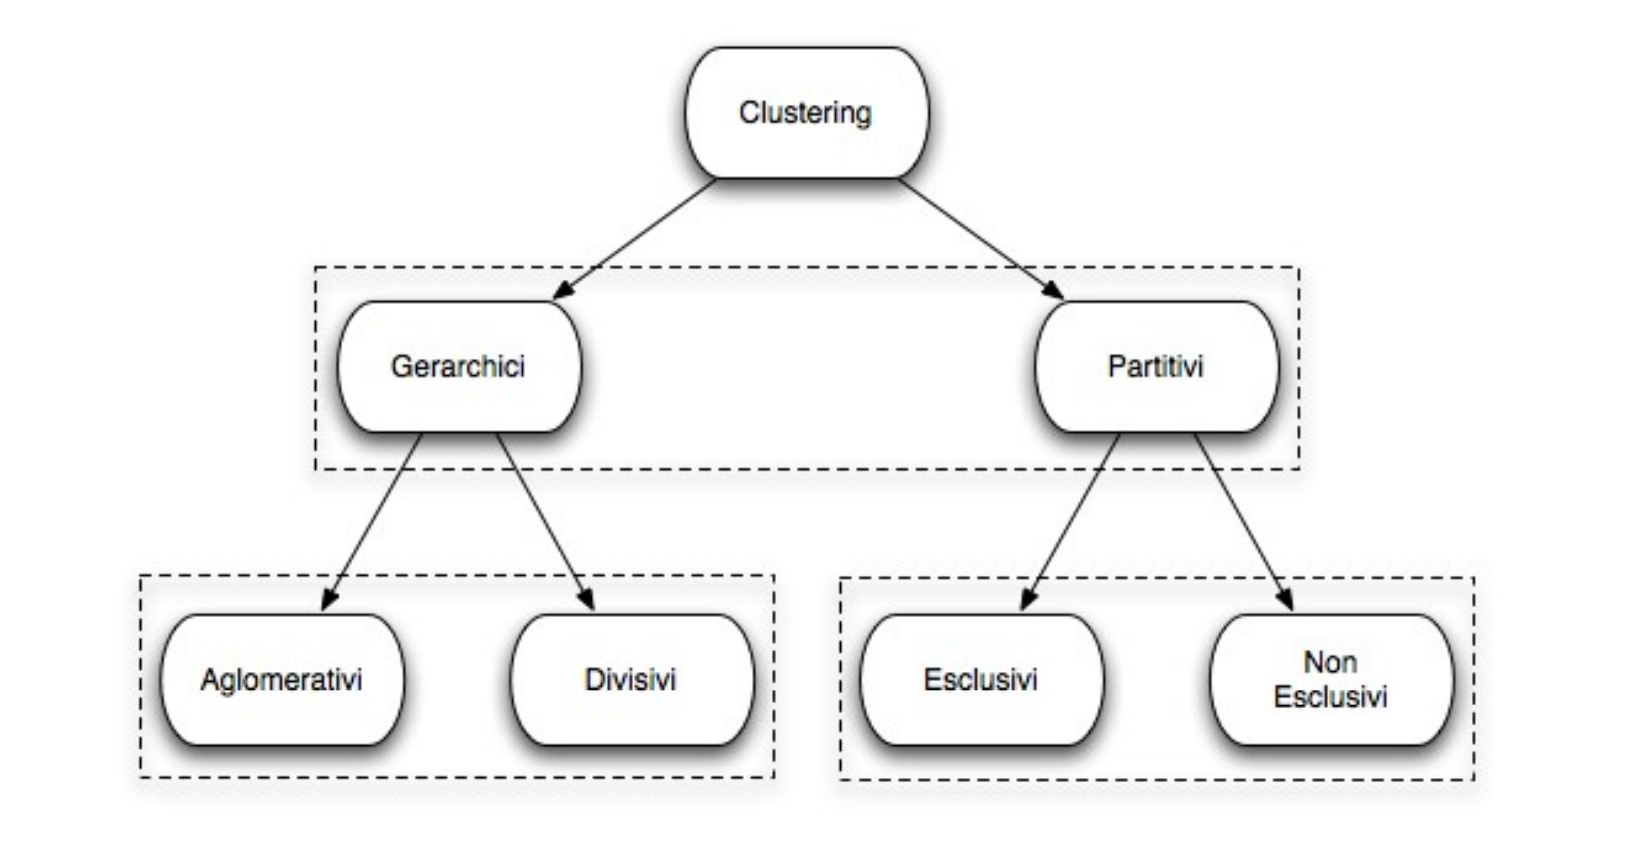
\includegraphics[scale = 0.3]{imm/cluster.PNG}
\end{figure}
Vediamo le due categorie principali esposte:
\begin{itemize}
    \item \textbf{Clustering gerarchico}, facendo questo tipo di clustering, quello che si va a eseguire, è il collocamento degli elementi in input in una struttura gerarchica ad albero, in cui le distanze tra nodi riflettono le similarità degli elementi. Gli elementi sono localizzati sulle foglie dell’albero.\\
    Ci sono alcuni vantaggi e svantaggi, infatti anche se sei si ha il vantaggio di avere una struttura singola, coerente e globale ed è un metodo intuitivo, purtroppo non ci sono esplicite partizioni nel cluster.
    \item \textbf{Clustering non gerarchico} mira a ripartire le $n$ unità della popolazione in $k$ gruppi, fornendo una sola partizione anziché una successione di partizioni tipica dei metodi gerarchici. Un esempio è il \textit{K-means}
\end{itemize}

\subsection{K-means}
Avevamo detto che è un metodo di cluster non gerarchico che opera per divisioni da un insieme iniziale. L'algoritmo prende in ingresso un intero $k$ e definisce iterativamente $k$ cluster che abbiano punti vicini in uno stesso cluster e punti distanti in cluster differenti. Si propone di minimizzare le distanze tra elementi e i centroidi dei clusters loro assegnati.
\subsubsection{Algoritmo K-means}(lavora solo con dati numerici)
Vediamo i vari step che vengono eseguiti durante l'utilizzo e l'implementazione di questo algoritmo:
\begin{enumerate}
    \item  Si fissano a caso $k$ centroidi iniziali di altrettanti cluster.
    \item  Per ogni individuo si calcola la distanza da ciascun centroide e lo si assegna al più vicino.
    \item  Per la partizione provvisoria così ottenuta si ricalcolano i centroidi di ogni cluster (media aritmetica).
    \item  Per ogni individuo si ricalcola la distanza dai centroidi e si effettuano gli eventuali spostamenti tra cluster.
    \item  Si ripetono le operazioni 3. e 4. finché si raggiunge il numero massimo di iterazioni impostate o non si verificano altri spostamenti.
\end{enumerate}
I vantaggi di questo algoritmo sono dati dal fatto che è di semplice implementazione e tempo di calcolo $\mathcal{O}(t\cdot k \cdot n)$ in cui $n$ è la cardinalità dell’insieme dei dati, $k$ è il numero di cluster e $t$ è il numero di iterazioni del ciclo (con $n \gg k, t$).\\
Si ha però una sensibilità rispetto alla scelta dei centroidi iniziali, non è possibile predire il numero di cluster non conoscendo i dati a priori, non esiste un $k$ ottimale e non ci sono proprietà che lo possano suggerire.\\
\subsubsection{Problematiche di K-means}
Con cluster con differenti dimensioni, con cluster con differenti densità, problematiche relative alle proprietà geometriche del cluster.
Una soluzione può essere l’utilizzo di un maggior numero di cluster a cui segue necessariamente una fase di unione in cluster più grandi.
\subsection{Misura di silhouette}
Data una distanza $d(i,j)$ tra due vettori o istanze $i,j$, in cluster con almeno due elementi al suo interno, è possibile calcolare:
\begin{itemize}
    \item \textbf{distanza media INTRA-cluster}: $a(i) = \displaystyle \frac{1}{|C_i| -1} \sum_{j \in C_i, i \neq j} d(i,j)$
    \item \textbf{distanza media INTER-cluster}: $b(i) = \displaystyle \min_{k \neq i} \frac{1}{|C_k|} \sum_{j \in C_k} d(i,j)$
    \item \textbf{silhouette} per un punto $i$: $s(i) = \displaystyle \frac{b(i) - a(i)}{\max \{a(i), b(i)\}}$\\
        Si vuole massimizzare la silhouette, massimizzando la distanza inter-cluster e minimizzando la distanza intra-cluster.
\end{itemize}
La media di $s(i)$, calcolata su tutti i punti di un cluster, è la misura di quanto strettamente sono raggruppati i punti nei cluster e quindi di quanto valido è il clustering effettuato.
infatti, in caso di troppi o troppo pochi cluster, come può accadere in seguito a una cattiva scelta di $k$ (numero di cluster), alcuni cluster avranno tipicamente una silhouette minore degli altri.
Quindi un plot delle silhouette potrebbe essere usato per determinare il numero di cluster da utilizzare per un determinato dataset.

\section{Reinforcement Learning}

\begin{figure}[H]
    \centering
    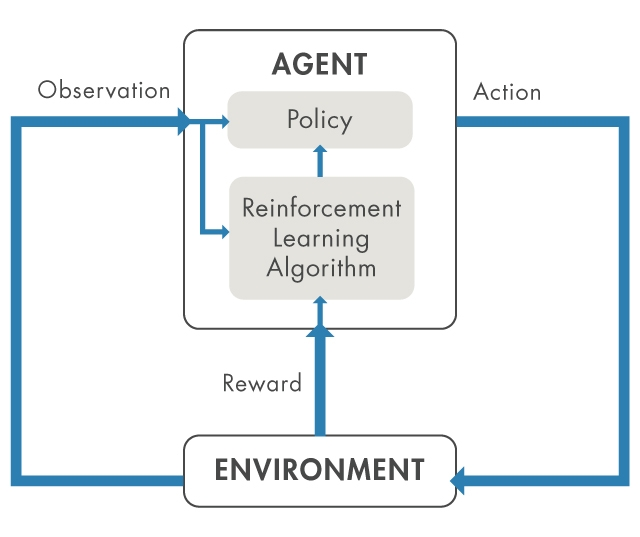
\includegraphics[scale=.4]{imm/reinforce.jpg}
    \caption{Diagramma riassuntivo del Reinforcement Learning}
\end{figure}

Normalmente, o almeno fin'ora, abbiamo visto che un errore implica un aggiustamento dell’ipotesi. L’errore è immaginato come una distanza tra comportamento presente e comportamento desiderato). Nel Reinforcement Learning, l’errore è rappresentato come premio o punizione per il comportamento; non c’è più la quantificazione di una distanza.\\ 

Al sistema viene associato un punteggio che dice se il sistema sta andando bene o male. E quindi di conseguenza i punti modificano le regole di comportamento del sistema.\\

Per esempio, all'interno di un gioco ci sono un ambiente, delle regole e delle interazioni che danno punti al nostro sistema. Normalmente nel Reinforcement Learning il sistema di punti è abbastanza generico perché non viene specificata la motivazione dietro al loro aumento o diminuzione. Non si sa esattamente come funziona l’ambiente, si sa solo interagire con esso, ovvero si possono compiere delle azioni nell’ambiente e farsi dire da quest’ultimo la nuova situazione dell’ambiente dopo l’azione.\\

Le decisioni di azione del sistema vengono prodotte da una politica interna di regole (policy) che si va via via a modificare tramite i punti ricevuti dall’ambiente stesso. L’algoritmo di Reinforcement Learning cambia la policy del sistema sulla base dei punti forniti dall’ambiente.

\subsection{Deep Learning}

Dalle reti neurali si passa a Deep Neural Net, ovvero reti neurali con più: strati (percettrone, backpropagation), algoritmi di discesa del gradiente, funzioni di attivazione, strumenti di regolazione comportando una maggior quantità di dati e una maggior potenza di calcolo.

\begin{figure}[H]
    \centering
    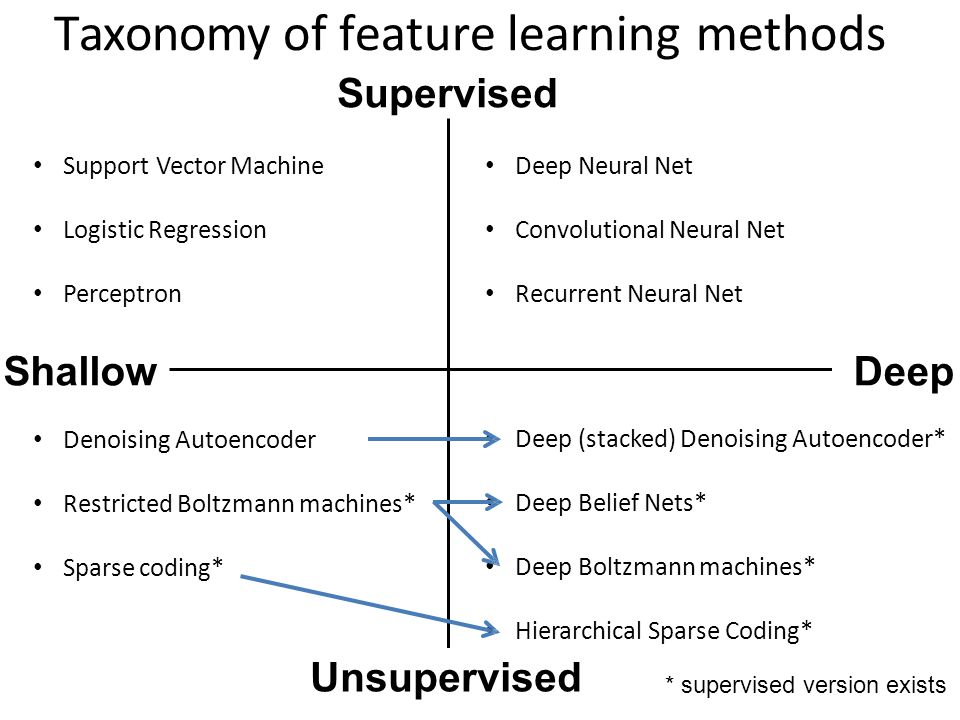
\includegraphics[scale=.4]{imm/deep-learn.jpg}
    \caption{Because some Deep Learning approaches are  considered to be Unsupervised -- it learns the features in the data  automatically (autoencoding)}
\end{figure}

La maggior parte degli algoritmi di Machine Learning non migliorano le proprie performance oltre una certa soglia di dati; mentre i nuovi metodi di deep learning riescono a sfruttare il continuo aumento dei dati, ottenendo un continuo miglioramento delle performance.\\

Nell’ambito dell’apprendimento su immagini, dal 2012 su è visto una sostanziale preferenza per i metodi di Deep Learning, a discapito di algoritmi più tradizionali.
Infatti gli algoritmi più tradizionali associavano alle immagini le feature corrispondenti in maniera manuale, mentre nel Deep Learning ciò avviene automaticamente tramite il sistema di apprendimento.\\

L’idea di un Multilayer Perceptron è quella di arricchire il comportamento delle reti aggiungendo layer e andando quindi in profondità. Ciò implica un aumento del numero di parametri (che potrebbe portare da overfitting) e un tempo di calcolo consistente. Sono quindi stati adottati alcuni rimedi per evitare questi effetti collaterali.\\

L’Autoencoder è una struttura (non profonda) shallow, non supervisionata che ha uno o più layer nascosti con un numero di unità nascoste minore del numero di feauture e che confronta i valori ottenuti in uscita con quelli forniti in ingresso. L’output è quindi in numero uguale al numero di feature in ingresso. \\
Questo modello produce quindi un errore (la distanza tra i vettori di input e output) che viene utilizzato per calcolare i pesi della rete.
Nell’hidden layer si ha una codifica (vettore di numeri in uno spazio a minor dimensioni) del dato di input.\\

Il Deep Learning è un set di algoritmi che imparano in layer, ovvero permettono al calcolatore di costruire una gerarchia di concetti compressi a partire da concetti più semplici.
Per esempio, per le immagini, si parte da un layer che contiene i pixel di input, passando a layer che man mano riconoscono linee, contorni, parti di oggetti fino all’identità degli oggetti.
Le feature vengono costruite automaticamente.

Struttura classica di apprendimento deep dedicato alle immagini
\begin{figure}[H]
    \centering
    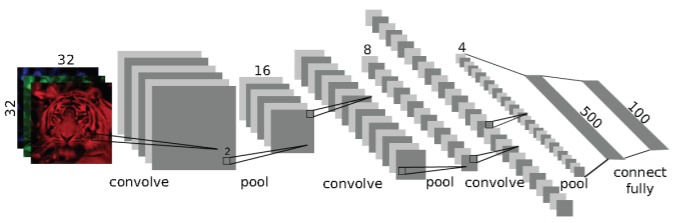
\includegraphics[scale=.8]{imm/imanges-deep.png}
\end{figure}

\textbf{\textit{Convoluzione}}\\

Al suo interno i neuroni sono connessi in un modo che evidenzia la struttura dei pixel nel campo visuale. Ciò è riprodotto nella connettività dei layer di certe reti. In origine un singolo neurone prendeva i segnali da tutti i pixel, ora invece un singolo neurone prende i segnali solo da una singola area di un’immagine. Un altro neurone prenderà i segnali da un’area spostata ma leggermente sovrapposta.\\

Ogni neurone quindi fa riferimento a una certa area-finestra dell’immagine e lo spostamento di questa finestra è ciò che viene definito convoluzione. La convoluzione rende evidente una struttura di adiacenza, non solo sui pixel di ingresso ma anche sui layer intermedi.\\

\textbf{\textit{Max pooling}}\\

Vede qual è il segnale più forte tra quelli ricevuti in ingresso e favorisce quello predominante. Il layer di pooling è formato da un gruppo di neuroni il cui segnale è trasformato nell’evidenza del più grande. Applicare l’operazione di pooling serve per ridurre l’immagine di input, riducendo quindi anche il numero di parametri.\\

Regolarizzare: combattere l’overfitting, sfumando lo spazio/ipotesi appreso.
Viene migliorata l’astrazione riducendo il numero di neuroni (dopo averli addestrati).
\section{Valutazione delle performance dei modelli supervisionati}

L’errore calcolato sul training set non è un buon indicatore delle performance su dati futuri (in quanto i nuovi dati probabilmente non saranno gli stessi dei dati di training).
\begin{itemize}
    \item \textit{Overfitting}: il modello si adatta troppo precisamente ai dati di training generando risultati scarsi su nuovi dati. Si ha un’alta complessità computazionale.
    \item \textit{Underfitting}: il modello si adatta poco ai (è inadatto per i) dati di training generando risultati scarsi su nuovi dati. Si ha una ridotta complessità computazionale.
\end{itemize}

\begin{figure}[H]
    \centering
    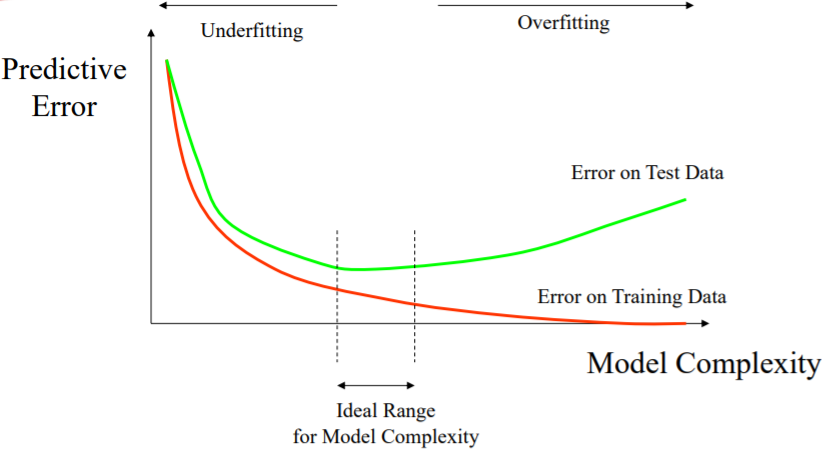
\includegraphics[scale=0.7]{imm/model_complexity.png}
\end{figure}

In mezzo si ha un buon compromesso tra accuratezza (e quindi tasso di errore) e complessità del modello.\\

Le tradizionali misure di performance per i problemi di classificazione sono le seguenti:
\begin{itemize}
    \item \textbf{success (successo)}: la classe di un’istanza è predetta correttamente.
    \item \textbf{error (errore)}: la classe di un’istanza non è predetta correttamente.
    \item \textbf{Error rate (tasso d’errore)}: proporzione di errori compiuti sull’intero set di istanze.
    \item \textbf{Accuracy (accuratezza)}: proporzione di istanze correttamente classificate su tutto il set dell’istanze.
\end{itemize}
Certamente ci sono altre modalità per calcolare la performance, ma questi sono quelli più gettonati/frequenti. 
% 
\begin{table}[H]
\centering
    \begin{tabular}{ll|l|l|}
        \cline{3-4}
        \multicolumn{2}{l}{\multirow{2}{*}{}} & \multicolumn{2}{|c|}{Predicted Class}               \\ \cline{3-4} 
        \multicolumn{2}{l}{}                  & \multicolumn{1}{|c }{Yes} & \multicolumn{1}{c|}{No} \\ \hline
        \multicolumn{1}{|l|}{\multirow{2}{*}{\begin{tabular}[c]{@{}l@{}}Actual  \\ class\end{tabular}}} & Yes & TP:true positive & Fn: False negative \\ \cline{2-4} 
        \multicolumn{1}{|l|}{}      & No      & FP: false positive       & TN: True negative       \\ \hline
    \end{tabular}
\end{table}

I metodi di machine learning solitamente tendono a minimizzare FP+FN. Nella pratica FP e FN possono avere costi diversi.\\

In un problema multiclasse, la matrice di confusione diventa:

\begin{table}[H]
\centering
\begin{tabular}{l|l|l|l|}
\cline{2-4}
 &
  $Class_1$ &
  $\cdots$ &
  $Class_n$ \\ \hline
\multicolumn{1}{|l|}{$Class_1$} &
  \begin{tabular}[c]{@{}l@{}}numero di elementi della classe 1 \\ predetti come elementi della classe 1\end{tabular}&
  $\cdots$ &
  \begin{tabular}[c]{@{}l@{}}numero di elementi della classe 1 \\ predetti come elementi della classe n\end{tabular} \\ \hline
\multicolumn{1}{|c|}{$\vdots$} &
   \multicolumn{1}{c|}{\vdots} &
  $\ddots$ &
  \multicolumn{1}{c|}{\vdots} \\ \hline
\multicolumn{1}{|l|}{$Class_n$} &
  \begin{tabular}[c]{@{}l@{}}numero di elementi della classe n \\ predetti come elementi della classe 1\end{tabular} &
  $\cdots$ &
  \begin{tabular}[c]{@{}l@{}}numero di elementi della classe n \\ predetti come elementi della classe n\end{tabular} \\ \hline
\end{tabular}
\end{table}

Gli elementi della diagonale sono i veri positivi, la riga di una classe è formata dai suoi falsi negativi e la colonna dai falsi positivi.

\subsection{Misure di performance tradizionali (globali)}

\begin{itemize}
    \item \textbf{Accuracy}: $\displaystyle \frac{TP+TN}{TP+TN+FP+FN}$
    \item \textbf{Precision}: $\displaystyle \frac{TP}{TP+FP}$	
    \item \textbf{Recall}: $\displaystyle \frac{TP}{TP+FN}$
    \item \textbf{F-measure}: $\displaystyle \frac{2 \cdot \text{Precision} \cdot \text{Recall}}{\text{Precision} + \text{Recall}}$
\end{itemize}

Nel caso di modelli multiclasse Precision, Recall e F-measure vengono calcolati specificatamente per una classe (non dell’intero modello). Solitamente si calcolano quindi Precision, Recall e F-measure per ogni classe e si calcola poi il valore medio.

\subsection{Misure di performance a livello di classe}

Data un’etichetta $l$ appartenente a un set $L$ di label:
\begin{itemize}
    \item \textbf{Precision}: $P(l) = \displaystyle \frac{\text{numero di istanze correttamente predette come  } l}{\text{numero di istanze predette come }l}$
    \item \textbf{Recall}: $R(l) = \displaystyle \frac{\text{numero di istanze correttamente predette come  } l}{\text{numero di istanze della classe }l}$
    \item \textbf{F-measure}: $F(l) = \displaystyle \frac{2 \cdot P(l) \cdot R(l)}{P(l) + R(l)}$
    \item \textbf{Macro-average}: $Perf^* = \displaystyle \frac{1}{|L|} \sum_{l=1}^{|L|} \cdot Perf(l)$, in questo caso tutte le classi sono equamente importanti
    \item \textbf{Micro-average}: $Perf^* = \displaystyle \sum_{l=1}^{|L|} \frac{|class(l)|}{\text{numero totale delle istanze}} \cdot Perf(l)$. \\ In questa situazione invece le classi predominanti (più corpose) sono le più importanti (media pesata)
\end{itemize}

Oltre ai metodi tradizionali si possono utilizzare le ROC curve. Le \textit{ROC (Receiver Operating Characteristic) curve} sono, in parole povere, delle curve che vengono plottate graficamente mostrano le performance di un classificatore ovvero la sua capacità discriminativa al variare di una determinata soglia.\\

Venie paragonato il rate dei veri positivi al rate dei falsi positivi al variare di una certa soglia.
\begin{figure}[H]
    \centering
    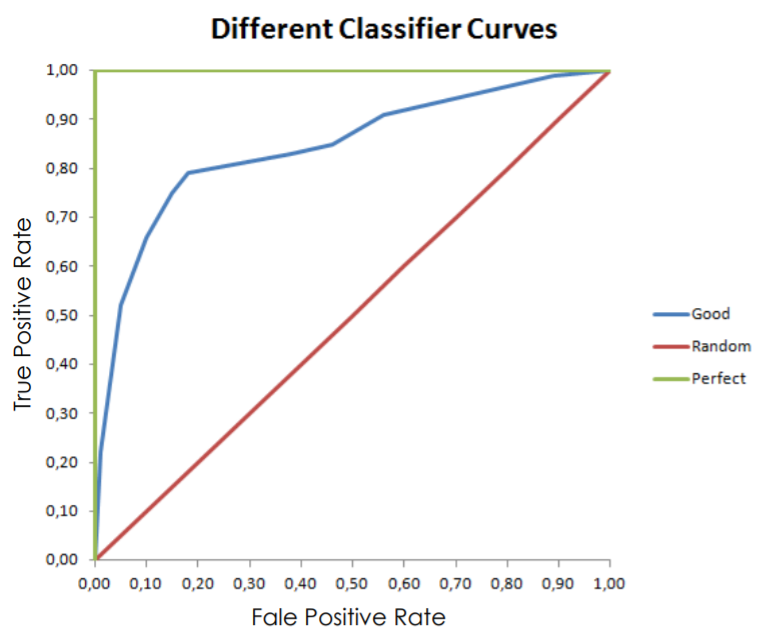
\includegraphics[scale=0.7]{imm/ROC_curve.png}
    \label{fig:roc_curve}
\end{figure}

Di curve ROC, ce ne è una per classe.

Ci sono inoltre le curve di apprendimento (\textit{learning curve}), queste curve ci mostrano invece come l’accuratezza (o un’altra misura di performance) cambia al variare della dimensione del campione. Sono uno strumento per evitare di andare in overfitting.\\

\begin{figure}[H]
    \centering
    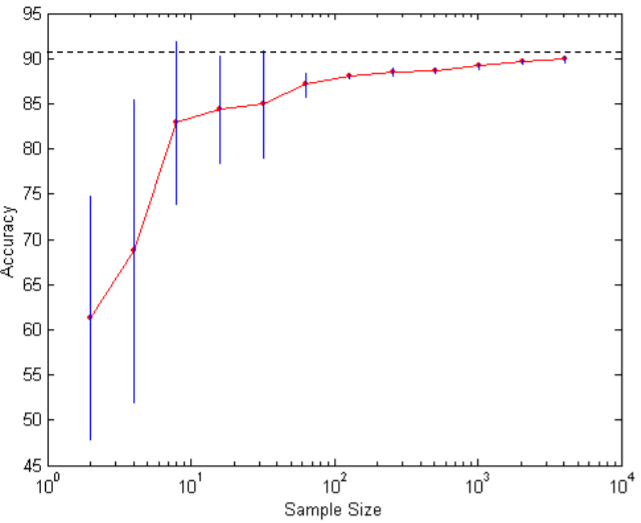
\includegraphics[scale=0.7]{imm/learning_curve.png}
    \label{fig:learning_curve}
\end{figure}
La linea rossa indica il variare dell’accuratezza al variare della dimensione dell’input. Le linee blu mostrano la varianza della performance.\\
A un certo punto al crescere dei dati non aumenta più la performance. \\

Se sono disponibili molti dati, e quindi molti esempi per ogni classe, è possibile convalidare il metodo di classificazione effettuando una semplice suddivisione randomica dei dati in training e test set (solitamente i dati sono divisi in $\frac{2}{3}$ training e l’$\frac{1}{3}$ test. \\
Si costruisce quindi il classificatore utilizzando il training set e lo si convalida usando il test set.\\

Una volta che si è effettuata la convalida, tutti i dati possono essere utilizzati per costruire il classificatore finale. \\
Generalmente, più dati vengono usati per il training e migliore è il classificatore e più dati vengono usati per il test e più accurata è la stima del tasso di errore. I dati di test non devono essere stati utilizzati per creare il classificatore e nemmeno per il tuning dei parametri.\\

La procedura corretta comprende quindi tre insiemi: i dati di training, i dati per la convalida (il validation set è utilizzato per ottimizzare i parametri) e i dati per il test.

\begin{figure}[H]
    \centering
    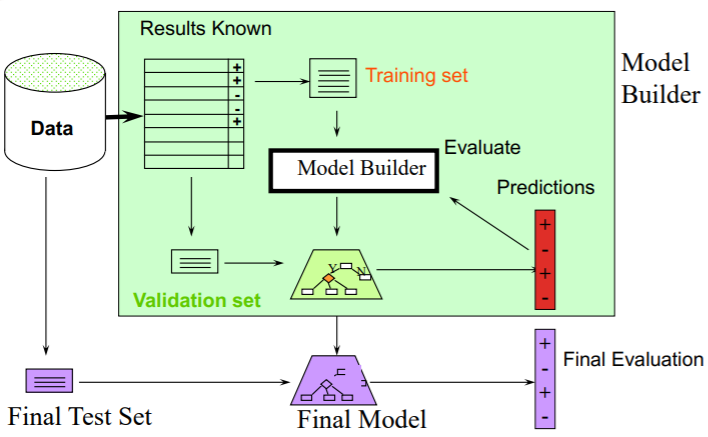
\includegraphics[scale=0.7]{imm/model_builder.png}
    \label{fig:model_builder}
\end{figure}

Nel caso in cui si abbia a che fare con un set di dati ristretto (con il rischio quindi che il training e il test set possano non essere rappresentativi) si utilizza un metodo detto \textit{repeated holdout}.\\

Nel metodo repeated holdout, viene ripetuto il processo di suddivisione in train e test set con diversi sottocampioni: ad ogni iterazione, viene selezionata casualmente una certa proporzione dal training set (possibilmente con stratificazione) e vengono pesate (attraverso una media) le stime d’errore in modo da ottenere una errore stimato globalmente equo.
Il problema è che i diversi test set possono contenere elementi ripetuti. Per risolver questo problema, quello che possiamo fare, è utilizzare una cross-validation.

\subsection{Cross-validation}
Metodo di repeated holdout che evita la sovrapposizione dei test set.
\begin{enumerate}
    \item I dati vengono suddivisi in $k$ sottoinsiemi di egual misura.
    \item Ogni sottoinsieme viene utilizzato a turno per testare e il resto viene usato per il training.
\end{enumerate}
Questo metodo viene chiamato \textit{k-fold cross-validation}. Spesso i sottoinsiemi vengono stratificati prima della cross-validation.

\begin{figure}[H]
    \centering
    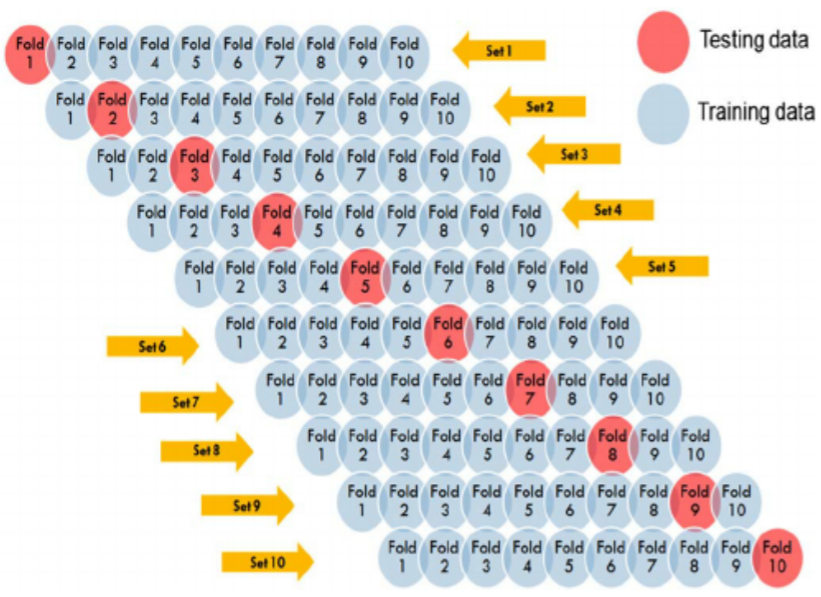
\includegraphics[scale=0.4]{imm/cross_validation.png}
    \label{fig:cross_validation}
\end{figure}

Nel caso in cui si voglia ottenere una matrice di confusione per l’intero 10-fold, si deve calcolare la matrice di confusione per ogni iterazione e poi sommarle.\\
Un metodo standard per la convalida che possiamo andare ad utilizzare è il \textbf{stratified \textit{ten}-fold cross-validation}.  
Con \textit{stratified}, intendiamo dire che la distribuzione delle istanze selezionate in relazione alla classe che dev’essere predetta in ogni fold, è simile alla distribuzione originale del dataset. La stratificazione riduce la varianza delle stime.\\

Una domanda lecita sarebbe chiedersi come mai \textbf{\textit{ten}-fold}. Di norma si usano 10 fold perché è stato dimostrata essere la miglior scelta per ottenere una stima accurata. Un metodo ancora migliore è il repeated stratified cross-validation nel quale la cross-validation è ripetuta $k$ volte e viene considerata la media dei risultati, al fine di ridurre al varianza.\\

\subsection{Bootstrap}
Ci sono altre tecniche, oltre alla cross validation, infatti come abbiamo detto la \textit{cross-validation} effettua il campionamento senza rimpiazzamento. Una stessa istanza, una volta selezionata, non può essere selezionata nuovamente per un determinato training/test set.\\
Mentre ci sono altre tecniche, come Bootstrap. In questa tecnica usa il campionamento con rimpiazzo per formare il training set. Suddivide un dataset di $n$ istanze $n$ volte con rimpiazzamento per formare un nuovo dataset di $n$ istanze che viene utilizzato come training set.Le istanze del dataset originale che non occorrono nel nuovo training set vengono utilizzate per il testing.\\

\subsubsection{0.632 Bootstrap}
Una particolare istanza ha una probabilità di $1 - \displaystyle \frac{1}{n}$ di non essere scelta.
Quindi la probabilità di finire nel test set è del: \[\left( 1- \displaystyle \frac{1}{n} \right)^n \approx e^{-1} = 0.368\]
Ciò significa che i dati di training conteranno approssimativamente il $63.2\%$ delle istanze.\\

Bootstrap tende a ridurre drasticamente la varianza, ma fornisce risultati con bias (tendono ad essere pessimistici).
È adatto a stimare la performance per dataset molto ridotti.

\subsubsection{Leave-One-Out Cross-Validation}
Una particolare forma di cross-validation che setta il numero di fold al numero delle istanze di training (con $n$ istanze di training, costruisce il classificatore $n$ volte). \\
Utilizza meglio i dati, senza coinvolgere sotto campionamenti casuali ma è molto costosa computazionalmente.\\

%%%%%%%%%%% Si aggiunge, dal laboratorio 10

Per sapere quanto si avvicina la stima del tasso di errore al tasso di errore effettivo, è possibile utilizzare gli intervalli di confidenza per capire meglio la proporzione che si sta considerando.\\

\textbf{\textit{Intervallo di confidenza (confidence interval)}}\\
Possiamo dire che $p$ appartiene a uno specifico intervallo con una specifica confidenza. A parità di tasso di errore stimato si sceglie il modello che garantisce un intervallo di confidenza più stretto (ovvero una minor variabilità del risultato).\\

\textbf{\textit{Significance test}}\\
I \textit{significance test} dicono quanto si può essere confidenti del fatto che ci sia effettivamente una differenza tra i risultati di due modelli. Abbiamo due modi per dirlo:
\begin{itemize}
    \item \textbf{Null hypothesis}hypothesis: non c’è una reale differenza.
    \item \textbf{Alternative hypothesis}: c’è una differenza.
\end{itemize}
Un test di significatività misura quanta evidenza c’è nel favorire il rigetto dell’ipotesi nulla.

\subsection{T di Student test}
Questo test ci dice se le medie di due campioni sono significativamente diverse. Consiste nel prendere campioni individuali dal set di tutte le possibili stime di cross-validation.

Si utilizza un t-test \textit{paired}: solo se i campioni individuali sono accoppiati (quindi se viene applicato a entrambi i modelli lo stesso cross-validation). È possibile applicarlo se i due modelli che si stanno testando stanno lavorando esattamente sulla stessa configurazione di fold (stesse istanze, stesse istanze nei fold e le istanze vengono processate esattamente nello stesso modo).\\

C’è una corrispondenza tra le predizioni dei due modelli.

\subsubsection{Calcolo del paired t-test}
Si considerano i campioni (gli elementi da confrontare, solitamente le predizioni) provenienti da un k-fold CV. Vengono normalizzati i dati per poter assumere di avere una distribuzione normale (media 0 e varianza 1). Con un campione dati abbastanza ampio possiamo sicuramente dire che la media di un seti di dati indipendenti è normalmente distribuito. Siano poi le stime di varianza delle medie date da $\frac{\sigma_x^2}{k}$ e $\frac{\sigma_y^2}{k}$, se $\mu_x$ e $\mu_y$ rappresentano le medie dei due campioni, allora: 
\[\displaystyle \frac{m_i - \mu_i} {\sqrt{\displaystyle \frac{\sigma_i^2}{k}}} \quad \mbox{ con } i \in \{x,y\}\],
Le media sono approssimamene normalmente distribuite con media uguale a 0 e varianza pari a 1.\\

Si calcolano $m_d = \mu_x - \mu_y$ (e si assume che anche questa sia distribuita normalmente) e $\sigma_d^2$ come la varianza della differenza. \\
A questo punto si calcola la statistica \[t = \displaystyle \frac{m_d}{\sqrt{\displaystyle \frac{\sigma_d^2}{k}}}\]
Dove $k$ è il numero di fold della $k$-fold cv(cross validation) (si assume che $m_d$ abbia una distribuzione di student con $k-1$ gradi di libertà), e la si usa per eseguire un t-test. Allora in ordine per eseguire il test eseguiamo i seguenti passi:
\begin{enumerate}
    \item Si fissa un livello di significatività $\alpha$ e se una differenza è significativa all’$\alpha\%$ allora c’è una possibilità del $(100-\alpha)\%$ che ci sia davvero una differenza.
    \item Si divide il livello di significatività per 2 perché il test è \textit{two-tailed}, e andiamoa a ritrovare il $z$ value associato al valore calcolato dalla $\alpha/2$.
    \item Se $t \leq -z$ o $t \geq z$ allora la differenza è significativa e quindi l’ipotesi nulla può essere rigettata.
\end{enumerate}

\subsection{Valutazione delle performance dei modelli non supervisionati}

Nella valutazione di una soluzione di clustering è bene considerare due fattori:
\begin{enumerate}
    \item \textit{Clustering tendency}: Bisogna verificare (prima del clustering) che i dati abbiano una tendenza (la clustering tendency) e che non contengano punti uniformemente distribuiti. Esistono due metodi per valutare la clustering tendency: 
        \begin{itemize}
            \item \textit{Hopkins statistic}: valuta la clustering tendency misurando la probabilità che un certo dataset sia generato da una distribuzione di dati uniforme, ovvero testa la spatial randomness dei dati. Sia $D$ un dataset real. La Hopkins statistic può essere calcolata come segue:
                \begin{enumerate}
                    \item Si campionano uniformemente $n$ punti ($p_1, \dots, p_n$) di $D$
                    \item  Si calcola la distanza $x_i$ da ogni punto reale al suo più vicino neighbor. 
                        Per ogni punto $p_i \in D$ si trova il più vicino punto $p_j$ e si computa la distanza tra i due $x_i = dist(p_i, p_j)$.
                    \item  Si genera un dataset simulato $randomD$ creato da una distribuzione uniforme e casuale di $n$ punti $q_1, \dots, q_n$ che abbia la stessa variazione del dataset originale $D$.
                    \item Si computa la distanza $y_i$ da ogni punto artificiale al più vicino punto reale.
                        Per ogni punto $q_i \in randomD$ si trova il più vicino punto $q_j \in D$ e si computa la distanza tra i due $y_i = dist(q_i, q_j)$.
                    \item Si calcola la Hopkins statistic $H$ come il rapporto tra la media delle distanze tra i punti più vicini in $randomD$ e la somma delle distanze medie tra i punti più vicini nel dataset reale e quello simulato.
                \end{enumerate}
                    \[\displaystyle H =  \displaystyle \frac{\displaystyle\sum_{i=1}^n{y_i}}{\displaystyle\sum_{i=1}^n{x_i} + \displaystyle\sum_{i=1}^n{y_i}} \]
            Un valore di $H$ maggiore di $0.75$ indica una clustering tendency con livello di confidenza al $90\%$.
            \item \textit{ Visual Assessment of cluster Tendency} (VAT) algorithm
                \begin{enumerate}
                    \item Si calcola la matrice di dissimilarità (dissimilarity matrix, DM) tra gli oggetti nel dataset usando la misura di distanza euclidea.
                    \item Si riordina la DM in modo tale che oggetti simili siano vicini tra di loro.
                       Questo processo crea una ordered dissimilarity matrix (ODM).
                    \item L’ODM è visualizzata come una ordered dissimilarity image (ODI) che l’output visuale del VAT.
                       \begin{figure}[H]
                            \centering
                            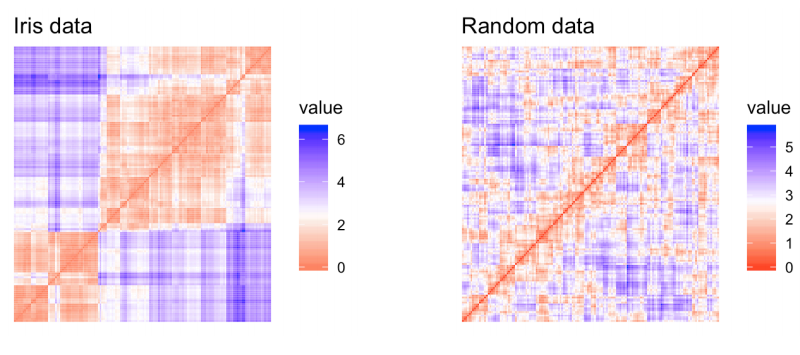
\includegraphics[scale=0.6]{imm/ODM.png}
                            \label{fig:odm}
                        \end{figure}
                \end{enumerate}
        \end{itemize}
    \item \textit{Clustering quality}: possibile utilizzare misure interne (within sum of square, silhouette) e misure esterne, se si hanno anche etichette associate alle istanze, (precision, recall, f-measure). \\
        Nel caso di misure esterne vige il criterio di maggioranza: si associa ad ogni cluster la classe a cui appartiene la maggioranza delle istanze del cluster.
\end{enumerate}
%%%%%%%%%%%%%%%%%%%%End of Lezioni
\setcounter{section}{0}
\newpage
\part{Esercitazione}
% %%%%%%%%%%%%%%%%%%%%Esercitazioni

\section{Esercitazione 1} 
\subsection{Terminolgia} 
\begin{itemize} 
    \item $X$, \textbf{spazio delle istanze}, ovvero la collezione di tutte le possibili \textbf{istanze} utili per qualche compito di \textit{learning}.
    \item $x\in X$, \textbf{istanza}, ovvero un singolo oggetto preso dallo \textbf{spazio delle istanze}. Ogni \textbf{istanza} è rappresentata tramite un vettore di attributi  
    \item $c$, \textbf{concetto}, $c\subseteq X$, ovvero un sottoinsieme dello \textit{spazio delle istanze} che descrive una \textit{classe} di oggetti (ovvero di istanze) alla quale siamo interessati per costruire un modello di \textit{machine learning}. 
    \item \textbf{esempio}, coppia formata da un’istanza e una sua possibile label che dovrebbe indicare la sua classe di appartenenza.
    \item $D=\{(x_1,f(x_1)),\ldots,(x_n,f(x_n))\}$, \textbf{training set} coppia formata da un’istanza e una sua possibile label che dovrebbe indicare la sua classe di appartenenza.
    \item $h$, \textbf{ipotesi}, $h\subseteq X$ 
    \item $H$, \textbf{spazio delle ipotesi} 
    \item $(x, f(x))$, \textbf{esempio}, ovvero prendo un'istanza e la vado ad etichettare con la sua classe di appartenenza. La funzione $f$ è detta \textbf{funzione target} 
    \item un \textbf{modello di machine learning} (dove \textit{machine learning} viene anche definito come lo studio di diverse strategie, più precisamente di ottimizzazione, per cercare ipotesi soddisfacenti/efficienti nello spazio delle ipotesi) è quindi l'\textit{ipotesi migliore}. 
    \item \textbf{linguaggio delle ipotesi}, è il linguaggio che definisce lo \textit{spazio delle ipotesi/modelli} 
    \item \textbf{cross validation}, ovvero ripeto $m$ volte la validazione su campioni diversi di input per evitare che un certo risultato derivi dalla fortuna 
    \item \textbf{concept learning}, problema di cercare all’interno di uno spazio delle ipotesi quelle funzioni che assumono valore all’interno dell’insieme $\to \{0,1\}$
    \item \textbf{funzione target}, spazio delle ipotesi/istanze $\to \{0,1\}$
    \item \textbf{ipotesi H}, ovvero una congiunzione $\land$ di vincoli sugli attributi. Tale ipotesi è \textbf{consistente}, ovvero è coerente con tutti gli esempi 
        \begin{itemize}
            \item \textbf{ipotesi più generale possibile}: per ogni attributo è ammesso ogni valore, non ci sono vincoli
            \item \textbf{ipotesi più ristrettiva possibile}: per nessun attributo non c’è alcun valore ammissibile .
        \end{itemize}
    \item \textbf{soddisfazione di un'ipotesi}: un'istanza $x$ soddisfa un'ipotesi $h$ sse tutti i vincoli espressi da $h$ sono soddisfatti dai valori di $x$ e si indica con: \[h(x)=1\]
\end{itemize}

General-to-specific relationship o More-general-than-or-equal-to relationship: definisce una relazione d’ordine parziale tra due ipotesi definite su uno stesso spazio delle ipotesi. $h_j$ è più generale o uguale a  $h_k$ ($h_k \geq h_j$) se e solo se $\forall x \in X$ (per ogni istanza nello spazio delle istanze) $h_k(x) = 1 \to h_j(x) = 1$

Un concetto deve appartenere allo spazio delle ipotesi considerato, affinché sia possibile trovare la strategia opportuna che lo rappresenti. 

Un istanza $x$ soddisfa un’ipotesi $h$  se e solo se tutti i vincoli espressi da $h$ sono soddisfatti grazie al valore di $x$. $x$ soddisfa $h \iff h(x) = 1$

Un’ipotesi è consistente con un determinato training set $D$ se per ogni esempio $x$ che appartiene a $D$ allora l’ipotesi applicata a $x$ è pari all’effettiva label/classe di $x$.
$$Consistent(h,D) = \forall \langle x,c(x) \rangle \in D \quad h(x) = c(x) $$ 

Cardinalità dello spazio delle istanze: prodotto delle cardinalità degli attributi. ($|X| = |A_1 x A_2 x \dots A_n|$)\\
Cardinalità dello spazio dei concetti: $2^{\textnormal{cardinalità dello spazio delle istanze}}$ \\
Cardinalità dello spazio delle ipotesi: Ogni ipotesi con un qualche $\varnothing$ è semanticamente equivalente, in quanto inconsistente. Quindi: (prodotto delle cardinalità $+$ 1(per il simbolo $?$) degli attributi) $+$ 1 per le ipotesi inconsistenti. 
\section{Esercitazione 2 - Find-S }
Siano appurate le conoscenze delle informazioni della lezione scorsa. Andiamo a utilizzare l'algoritmo Find-S.

\subsection{Esercizio 1}

\begin{table}[h]
\centering
\begin{tabular}{|l|l|l|l|l|l|}
\hline
\textbf{Ex Numb} & \textbf{$A_1$} & \textbf{$A_2$} & \textbf{$A_3$} & \textbf{$A_4$} & \textbf{Label} \\ \hline
\textbf{$x_1$}     & 1            & 0            & 1            & 0            & 1              \\ \hline
\textbf{$x_2$}     & 0            & 1            & 0            & 0            & 0              \\ \hline
\textbf{$x_3$}     & 1            & 0            & 1            & 1            & 0              \\ \hline
\textbf{$x_4$}     & 0            & 0            & 0            & 0            & 1              \\ \hline
\textbf{$x_5$}     & 0            & 0            & 1            & 0            & 1              \\ \hline
\end{tabular}
\end{table}

Seguendo l'algoritmo find-s, dobbiamo inizializzare h come ipotesi più specifica, nel nostro caso\\  $S = \{\langle \varnothing \, , \varnothing \, ,\varnothing \, ,\varnothing \, \rangle\}$. Ci si presenta il primo esempio $x_1 = (1,0,1,0)$ e la sua corrispettiva label $t(x_1) = 1$. Questo non soddisfa il vincolo di S, e quindi in $S$ faccio il \textit{replace} del valore del primo attributo di $x_1$ con quello di $S$. Visto che $S$ è però l'ipotesi più specifica dovrò farlo per tutti i vincoli, ottenendo che $S$ diventa, di fatto, una copia di $x_1$: $S = \{\langle 1,0,1,0\rangle\}$ \\
Si presenta la seconda ipotesi $x_2 =(0,1,0,0)$,che ha label pari a 0, quindi $t(x_2)=0$. Essendo un esempio negativo viene ignorato dall'algoritmo, lasciando inalterato $S$.\\Analogo ragionamento per il terzo esempio.\\
Per quanto riguarda invece il quarto esempio $x_4 = (0,0,0,0)$, con la label $t(x_4) = 1$, varierà la nostra S. 
Dove si ha lo stesso valore lo tengo in $S$, altrimenti pongo il caso generico $?$, ci porta quindi ad avere una $S$ nella seguente forma: $S = \{\langle ?,0,?,0\rangle\}$ \\
Si presenta il quinto esempio $x_5=(0,0,1,0)$ che ha label 1, quindi $t(x_5)=1$. Procedo come sopra e ottengo, infine: $S=\{\langle ?,0,?,0\rangle\}$. \\ \newline Si arriva quindi a dire che $S=\{\langle ?,0,?,0\rangle\}$ è la nuova ipotesi più specifica che verrà restituita dall'algoritmo \textbf{find-S}.

\subsection{Esercizio 2}
Ipotesi finale restituita da algoritmo find-s, cosa devo fare: $S=\{\langle ?,0,?,0\rangle\}$\\
Attraverso tre esempi positivi $t(x_i) = 1$, e due negativi $t(x_i) = 0$, raggiungere alla ipotesi dichiarata S.\\

\begin{table}[h]
\centering
\begin{tabular}{|l|l|l|l|l|l|}
\hline
\textbf{Ex Numb} & \textbf{$A_1$} & \textbf{$A_2$} & \textbf{$A_3$} & \textbf{$A_4$} & \textbf{Label} \\ \hline
\textbf{$x_1$}     & 1            & 0            & 1            & 1            & 1              \\ \hline
\textbf{$x_2$}     & 0            & 1            & 0            & 0            & 0              \\ \hline
\textbf{$x_3$}     & 1            & 0            & 1            & 1            & 1              \\ \hline
\textbf{$x_4$}     & 0            & 0            & 0            & 0            & 0              \\ \hline
\textbf{$x_5$}     & 0            & 0            & 0            & 0            & 1              \\ \hline
\end{tabular}
\end{table}
Con gli ultimi due che rappresentano, in un contesto reale, un \textbf{errore} e un \textbf{rumore}, in quanto gli stessi valori portano ad avere le due \textit{label} opposte, si ha quindi inconsistenza. Sono infatti detti \textbf{esempi inconsistenti} e vengono completamente ignorati da \textbf{find-S}.

L'algoritmo riporta alcuni difetti:
\begin{itemize} 
    \item potrebbero esserci altre ipotesi consistenti rispetto a quella in output 
    \item i training set inconsistenti possono ingannare l'algoritmo 
\end{itemize} D'altro canto: 
\begin{itemize} 
    \item garantisce in output l'ipotesi più specifica consistente con gli esempi positivi 
    \item l'ipotesi finale è consistente anche con gli esempi negativi, a patto che il \textit{target concept} sia contenuto in $H$ e che gli esempi siano corretti 
\end{itemize}

\section{Esercitazione 2}
\subsection{Percettrone}
Un percettrone si basa su un’unica unità di calcolo che riceve un input e attraverso una funzione soglia valorizza l’uscita facendole assumere un valore 1 o -1.\\
Una rete neurale, e quindi anche l’unità di calcolo del percettrone, riceve in ingresso un segnale che viene scalato da alcuni pesi (parametri apprendibili dalla rete che devono essere fittati in modo corretto per diminuire la funzione di errore).\\

Il segnale di ingresso ha come prima componente un’unità che poi verrà scalata dal corrispettivo peso. 
La somma dei pesi moltiplicati per il segnale d’ingresso costituisce il potenziale di attivazione, dal quale viene determinato tramite la funzione a soglia il valore in output: se la sommatoria è maggiore di 0, l’output sarà 1, altrimenti -1. 
Nel percettrone, si considera come errore la differenza tra l’output (1 o -1) e il corrispettivo valore associato all’istanza in ingresso (label dell’esempio corrente).
L’errore viene poi fattorizzato nella variazione dei pesi $\Delta$ che viene sommata al peso attuale per generare il nuovo peso.

\begin{figure}[H]
    \centering
    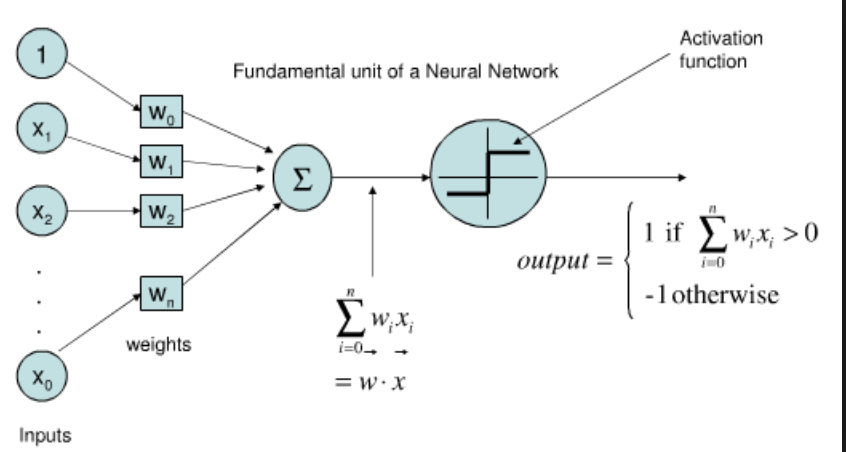
\includegraphics[scale = 0.8]{imm/perceptron_1.png}
\end{figure}

\textbf{Algoritmo}\\
Per esempio $(x,t)$ con $x$ istanza e $t$ etichetta target.
\begin{enumerate}
    \item Si computa $y = step(f(x))$
    \item  $w \leftarrow w + \alpha(t-y)x$, dove $\alpha$ è il learning rate
\end{enumerate}
Se l’output: 
\begin{itemize}
    \item corrisponde con il target: $(t-y) = 0$ e i pesi non vengono aggiornati 
    \item $=1$ e il target è $0$: l’input (scalato da $\alpha$) è sottratto dal vettore dei pesi.
    \item $=0$ e il target è $1$: l’input (scalato da $\alpha$) è aggiunto al vettore dei pesi.
\end{itemize}
\subsection{Adaline}

Simile al percettrone ma gli errori vengono valutati nel continuo (tramite una funzione di attivazione lineare che ha come argomento il potenziale).
Mentre nel percettrone l’output binario serviva per il calcolo dell’errore e l’aggiornamento dei pesi (per imparare i coefficienti del modello vengono usate le label); in Adaline l’errore viene calcolato su un valore continuo consentendo quindi di dire anche di quanto ci si è sbagliati (per imparare i coefficienti del modello si usano i valori continui predetti)
\begin{figure}[H]
    \centering
    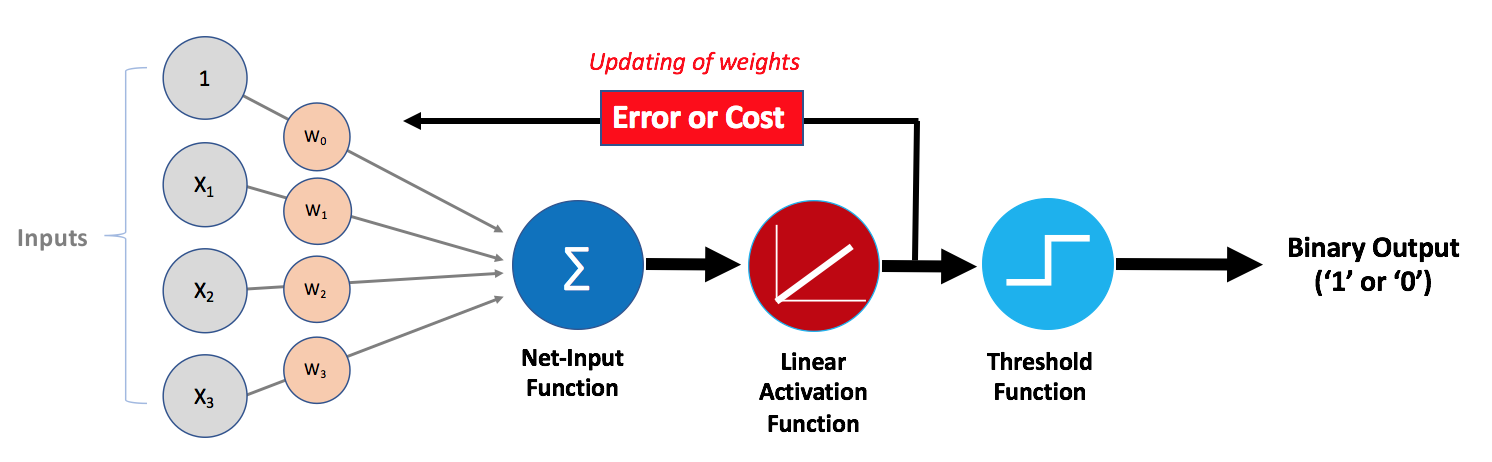
\includegraphics[scale = 0.5]{imm/perceptron_2.png}
\end{figure}

\textbf{Algoritmo}\\
Per esempio $(x,t)$ con $x$ istanza e $t$ etichetta target:
\begin{enumerate}
    \item Si computa $z = f(x)$
    \item  $w \leftarrow w + \alpha(t-z)x$, dove $\alpha$ è il learning rate
\end{enumerate}

Ciò equivale a applicare la regola del gradiente discendente alla regressione lineare (con lo squared error loss).
Infatti, la derivata di $(z-t)^2$ è $2(z-t)$ e il fattore costante $2$ può essere omesso dal momento che si sta usando $\alpha$ come learning rate per modulare quanto ogni update modifica i pesi correnti.

\begin{figure}[H]
    \centering
    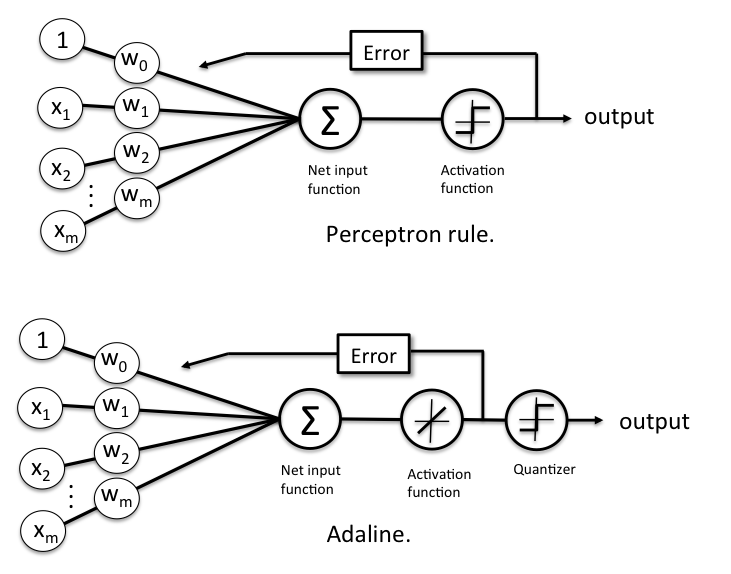
\includegraphics[scale = 0.8]{imm/perceptron_3.png}
\end{figure}

\begin{figure}[H]
    \centering
    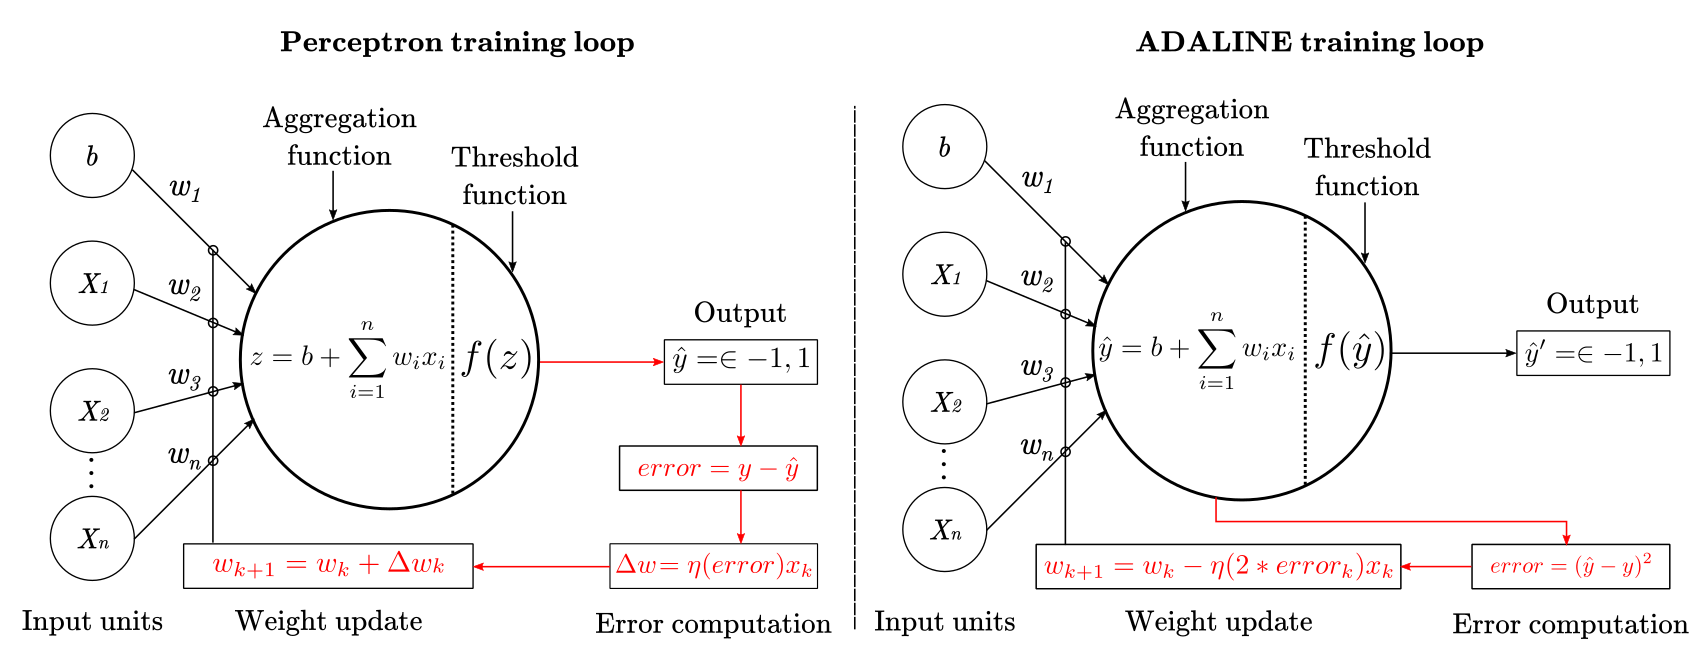
\includegraphics[scale= 0.6]{imm/adaline-math.png}
\end{figure}

\subsubsection{Separazione lineare}
Un set di punti linearmente separabili usa gli iperpiani per effettuare la separazione.

Le reti neurali dette feedforward neural networks prevedono diversi livelli computazionali: il segnale d’ingresso passa attraverso vari livelli (layers) in ognuno dei quali viene calcolata una funzione prendendo in input gli output della funzione del layer precedente.

\section{Bayes concept learning}
\subsection{RECAP}
Avevamo detto che, mentre in un normale approccio di learning si andava a cercare l'ipotesi migliore all'interno dello spazio $H$ . Nel approccio Bayesiano si va a cercare l'ipotesi più probabile $h$. Si ha quindi un approccio probabilistico, si ha una probabilità a priori denotata come $P(h)$. Si hanno inoltre:
\begin{itemize}
    \item $P(D)$, questa viene denotata come evidenza 
    \item $P(D|h)$, una probabilità condizionata, rappresenta la probabilità di osservazione di alcune informazioni conoscendo una determinata ipotesi
\end{itemize}
Siano rispettivamente 
\begin{itemize}
  \item $D$ è il dataset
  \item $\theta$ che per noi è l'ipotesi (o grado di incertezza che si ha in merito all'ipotesi?)
  \item $P(\theta|D)$ che è la distribuzione a posteriori, di una ipotesi 
  \item $P(\theta)$ è la distribuzione a priori
  \item $P(D|\theta)$ è la verosimiglianza
  \item $P(D)$ è l'evidenza
\end{itemize}
Andioamo a riprendere la formula che rappresenta l'approccio di Bayes:
\[P(\theta|D)=\frac{P(D|\theta)P(\theta)}{P(D)}\]
Sapendo che: 
\[P(D)=\sum_i P(D, \theta_i)=\sum_i P(D|\theta_i)P(\theta_i)\]
Spesso $P(D)$ è difficile da calcolare attraverso una sommatoria, richiederebbe molto tempo per essere calcolata, quindi molto spesso vengono considerate solamente la probabilità a posteriori è considerata. Questo ci va bene perché $P(D)$ è invariante rispetto al valore dell'ipotesi e quindi possiamo benissimo rimuoverlo nel calcolo in quanto non influisce sulla probabilità a posteriori:
\[P(\theta_i|D)\varpropto P(D|\theta_i)P(\theta_i)\]
(si ricorda che $\varpropto$ indica \textbf{proposizionale a} quindi che due cose sono uguali al più di una costante)\\ Ricordiamo inoltre che la massima ipotesi a posteriori è:
\begin{equation*}
    \begin{split}
        h_{MAP}&=\operatorname*{argmax}_{h\in H}P(h|D) \\
        & = \operatorname*{argmax}_{h\in H}\frac{P(D|h)P(h)}{P(D)} \\
        & = \operatorname*{argmax}_{h\in H}P(D|h)P(h)
    \end{split}
\end{equation*}
Se si sa che anche la conoscenza a priori è ininfluente, essendo distribuita seconda una distribuzione uniforme, e si parla di ipotesi di massima verosimiglianza:
\[h_{ML}=\operatorname*{argmax}_{h\in H}P(D|h)\]
L'approccio di Bayes nel machine learning è abbastanza oneroso, dovendo
calcolare tutte le probabilità a posteriori di ogni ipotesi (se $H$ è grande diventa molto costoso).

\subsection{Naive recap}
Ricordiamo che per Naive Bayes si ha, avendo una sequenza $d_1,d_2\ldots d_n$ di osservazioni: 
\begin{equation*}
    \begin{split}
        h_{MAP}&=\operatorname*{argmax}_{h\in H}P(h|d_1,d_2\ldots d_n) \\
        &=\operatorname*{argmax}_{h\in H}\frac{P(d_1,d_2\ldots d_n|h)P(h)}{P(D)} \\
        &\varpropto\operatorname*{argmax}_{h\in H}P(d_1,d_2\ldots d_n|h)P(h)
    \end{split}
\end{equation*}
Per semplificare, tramite naive Bayes,si può assumere:
\[P(d_1,d_2\ldots d_n|h)=\prod_iP(d_i|h)\]
ovvero indipendenza condizionata (dicendo che un valore $d:i$ è indipendente da
un qualunque $d_j$) e quindi si ha, sostituendo:
\[h_{MAP}=\operatorname*{argmax}_{h\in H}P(h)\prod_iP(d_i|h)\]
\section{Kernel/SVM \& KMeans}
\subsection{Iperpiano}
L'iperpiano, a seconda dello spazio di rappresentazione, ha diverse rappresentazioni, infatti in uno spazio euclideo a $n$ dimensioni, è un sottoinsieme dello spazio a $n-1$ dimensioni, che divide lo spazio in due parti non connesse. Si tratta di un set di punti che soddisfa l’equazione: $\bold{w} \cdot \bold{x} + b = 0$.
\begin{itemize}
    \item In una dimensione, è un punto.
    \item In tre dimensioni, è un piano.
    \item 
In più di tre dimensioni, si chiama iperpiano.
\end{itemize}

Nello spazio a due dimensioni:
\begin{equation*}
    \begin{split}
        \bold{w} \cdot \bold{x} + b = 0 & \implies w_0 x + w_1 y + b = 0\\
        & \implies w_1 y = -w_0 x - b\\
        & \implies y = \displaystyle -\frac{w_0}{w_1}x - \frac{b}{w_1}
    \end{split}
\end{equation*}
Ponendo $a = \displaystyle -\frac{w_0}{w_1}$ e $c = \displaystyle - \frac{b}{w_1}$, si ottiene \[y = ax + c\]

Se un punto si trova sull’iperpiano, $\bold{w} \cdot \bold{x} + b$ è uguale a zero, altrimenti produce un risultato $\neq 0$. 
\subsection{Classificazione usando un iperpiano}
Quello che siamo intenti a capire è: quale iperpiano è il miglior iperpiano possibile? Per dare risposta alla nostra domanda ci basiamo sulla classificazione, denotiamo quindi la nostra idea con il seguente esempio. L'esempio racchiude i concetti base.\\

È possibile definire la funzione di un’ipotesi $h$ come: 
$h(\bold{x_i}) = 
    \begin{cases} 
        + 1 & \text{ if }\ \bold{w} \cdot \bold{x_i} + b \geq 0 \\ 
        - 1 & \text{ if }\ \bold{w} \cdot \bold{x_i} + b < 0
    \end{cases}
$\\

che equivale a $h(\bold{x_i}) = \text{sign}(\bold{w} \cdot \bold{x_i} + b)$.\\
\subsubsection{Classificazione sicura e margine}
Dato un esempio di training $(x,y)$ e un iperpiano definito da un vettore $\bold{w}$ e un bias $b$, si può computare il numero $\beta = \bold{w} \cdot \bold{x} + b$ per sapere quanto dista il punto dall’iperpiano.\\
Se si moltiplica $\beta$ per il valore di $y$, si ottiene il margine funzionale $f = y \times \beta = y (\bold{w} \cdot \bold{x} + b)$, dove il simbolo di $f$ sarà sempre positivo se i punti sono classificati correttamente e negativo altrimenti. Questo lo facciamo perché la definizione che abbiamo dato di $\beta$ da sola non ci basta per la decisione dell'iperpiano.\\
Infatti, se $y = 1$, per far sì che il margine funzionale sia ampio (e quindi la predizione confidente e corretta), serve che $\bold{w} \cdot \bold{x} + b$ sia un numero positivo grande.\\
Se $y = -1$, per far sì che il margine funzionale sia ampio, serve che $\bold{w} \cdot \bold{x} + b$ sia un numero negativo grande. \\
Inoltre, se $y (\bold{w} \cdot \bold{x} + b) > 0$, allora la predizione su $(x,y)$ è corretta.\\

Margine funzionale rispetto all’$i$-esima osservazione: $\hat \gamma^{(i)} = y^{(i)}(\bold{w^T x} + b)$.\\
Margine funzionale rispetto all’intero insieme di esempi: $\displaystyle \hat \gamma = \operatorname*{min}_{i = 1, \dots, m}\hat \gamma^{(i)}$.\\

La predizione della classe dipende solo dal segno di $h$ (infatti $h(\bold{x_i}) = \text{sign}(\bold{w} \cdot \bold{x_i} + b)$).
Utilizzare multipli di $\bold{w}$ e di $b$, permette di aumentare la larghezza del margine ma in realtà ciò non implica una maggior confidenza nelle predizioni in quanto $h(\bold{wx} + b) = h(a \bold{wx} + ab)$ (hanno lo stesso segno) e $(\bold{w}, b)$ e $(a\bold{w}, ab)$ rappresentano lo stesso iperpiano.

Dato che per lo stesso iperpiano si voleva considerare un margine di confidenza maggiore, quello che possiamo fare per evitare che questo accada è di andare a utilizzare al posto del margine funzionale, il margine geometrico. Quest'ultimo ci restituisce una misura invariante allo scaling dei parametri.
Denotiamo il margine geometrico attraverso la formula \[\gamma^{(i)} = y^{(i)} \left(\left(\displaystyle \frac{w}{||w||}\right)^T x^{(i)} + \frac{b}{||w||}\right)\]
ottenuto dividendo il margine funzionale per $||w||$.
Il margine funzionale viene comunque utilizzato come funzione di test per verificare se un determinato punto è stato classificato correttamente.\\

Margine geometrico rispetto all’$i$-esima osservazione: $\gamma^{(i)} = y^{(i)} \left(\left(\displaystyle \frac{w}{||w||}\right))^T x^{(i)} + \frac{b}{||w||} \right)$. \\
Margine geometrico rispetto all’intero insieme di esempi: $\displaystyle \gamma =  \min_{i = 1, \dots, m} \gamma^{(i)}$.\\

Idea per scegliere l’iperpiano separatore: scegliere quello che massimizza il margine da entrambe le classi del training set. Ciò significa massimizzare la distanza tra i punti più vicini di ogni classe (il minimo dei margini geometrici tra tutti gli esempi). Il classificatore separerà quindi gli esempi di training positivi dai negativi con un gap.
\subsection{SVM}
Ha come scopo quello di massimizzare il minimo margine geometrico. L’SVM cerca l’iperpiano che è il più distante possibile dai membri di ogni classe.

\subsection{Metodi di mapping}
Se non si riesce a separare gli esempi positivi dai negativi in uno spazio a dimensioni minori usando un iperpiano, è possibile mappare tutto in uno spazio dimensionale a dimensioni maggiori nel quale si riesce a separarli.

\subsection{Kernel}
Siano $X$ lo spazio delle istanze e $F$ lo spazio delle feature.
Una funzione $k : X \times X \to \mathbb{R}$ è un kernel valido se esiste una \textit{feature map} $\phi : X \to F \mbox{ tale che }$ \[k(x, z) = \langle\phi(x), \phi(z)\rangle, \forall x, z \in X\]
Ha come argomento una coppia di punti nello spazio originale e ha la caratteristica di poter essere rappresentata nello spazio di arrivo (spazio delle feature) un prodotto interno. Il prodotto interno in uno spazio euclideo è il prodotto scalare tra due vettori (ovvero di due featue che sono il risultato del mapping). Nello specifico, un kernel valido opera il prodotto interno tra due feature che sono il risultato del mapping nello spazio delle feature di due istanze dello spazio originale.\\

Il kernel può essere pensato come una similarità tra oggetti.\\

Un kernel definisce un prodotto interno \textit{(dot product)} tra vettori. Uno spazio vettoriale che ha un prodotto interno, ha una norma della forma: $||x|| = \sqrt{\langle x, x \rangle}$. Se si ha una norma, si ha una distanza $d(x,y) = ||x-y||$. Quindi il kernel misura la similarità tra due oggetti come l‘inverso della loro distanza.\\

Dato un kernel $k$ e un insieme $S = \{x_1, \dots, x_n\}$, si può definire la \textit{kernel matrix} corrispondente: \[G_{i,j} = \langle \Phi(x_i), \Phi(x_j) \rangle = k(x_i, x_j)\]

Molti algoritmi interagiscono con i dati tramite prodotti interni.
Quindi se si sostituisce $x \cdot z$ con $k(x, z)$, essi agiranno implicitamente come se i dati appartenessero a uno spazio $\Phi$ a dimensioni maggiori. 

\subsection{Strategia di kernel o kernellizzazione}
Dal momento che è possibile costruire una funzione $k(x,z)$, tale che \[k(x,z) = \langle \Phi(x), \Phi(z)\rangle_H \mbox{ con }\Phi : X \to H\] allora durante l’addestramento ogni volta che si deve computare $\langle \Phi(x), \Phi(z) \rangle_H$ basterà valutare $k(x,z)$; infatti non c’è bisogno di applicare effettivamente la funzione $\Phi$. In questo modo, si dice che la trasformazione esiste solo implicitamente.\\

Un metodo è \textit{kernellizzato} se ogni vettore delle feature $\psi(x)$ appare solo dentro un prodotto interno con un altro vettore delle feature $\psi(z)$. Ciò si applica sia ai problemi di ottimizzazione che alla funzione di predizione.

\textit{ESERCIZIO 1 SUL FOGLIO}
%%%%%%%%%%%%%%%%%%%%End of Esercitazioni
\end{document}
